
%% bare_conf.tex
%% V1.3
%% 2007/01/11
%% by Michael Shell
%% See:
%% http://www.michaelshell.org/
%% for current contact information.
%%
%% This is a skeleton file demonstrating the use of IEEEtran.cls
%% (requires IEEEtran.cls version 1.7 or later) with an IEEE conference paper.
%%
%% Support sites:
%% http://www.michaelshell.org/tex/ieeetran/
%% http://www.ctan.org/tex-archive/macros/latex/contrib/IEEEtran/
%% and
%% http://www.ieee.org/

%%*************************************************************************
%% Legal Notice:
%% This code is offered as-is without any warranty either expressed or
%% implied; without even the implied warranty of MERCHANTABILITY or
%% FITNESS FOR A PARTICULAR PURPOSE!
%% User assumes all risk.
%% In no event shall IEEE or any contributor to this code be liable for
%% any damages or losses, including, but not limited to, incidental,
%% consequential, or any other damages, resulting from the use or misuse
%% of any information contained here.
%%
%% All comments are the opinions of their respective authors and are not
%% necessarily endorsed by the IEEE.
%%
%% This work is distributed under the LaTeX Project Public License (LPPL)
%% ( http://www.latex-project.org/ ) version 1.3, and may be freely used,
%% distributed and modified. A copy of the LPPL, version 1.3, is included
%% in the base LaTeX documentation of all distributions of LaTeX released
%% 2003/12/01 or later.
%% Retain all contribution notices and credits.
%% ** Modified files should be clearly indicated as such, including  **
%% ** renaming them and changing author support contact information. **
%%
%% File list of work: IEEEtran.cls, IEEEtran_HOWTO.pdf, bare_adv.tex,
%%                    bare_conf.tex, bare_jrnl.tex, bare_jrnl_compsoc.tex
%%*************************************************************************

% *** Authors should verify (and, if needed, correct) their LaTeX system  ***
% *** with the testflow diagnostic prior to trusting their LaTeX platform ***
% *** with production work. IEEE's font choices can trigger bugs that do  ***
% *** not appear when using other class files.                            ***
% The testflow support page is at:
% http://www.michaelshell.org/tex/testflow/



% Note that the a4paper option is mainly intended so that authors in
% countries using A4 can easily print to A4 and see how their papers will
% look in print - the typesetting of the document will not typically be
% affected with changes in paper size (but the bottom and side margins will).
% Use the testflow package mentioned above to verify correct handling of
% both paper sizes by the user's LaTeX system.
%
% Also note that the "draftcls" or "draftclsnofoot", not "draft", option
% should be used if it is desired that the figures are to be displayed in
% draft mode.
%
\documentclass[conference]{IEEEtran}
% Add the compsoc option for Computer Society conferences.
%
% If IEEEtran.cls has not been installed into the LaTeX system files,
% manually specify the path to it like:
% \documentclass[conference]{../sty/IEEEtran}





% Some very useful LaTeX packages include:
% (uncomment the ones you want to load)


% *** MISC UTILITY PACKAGES ***
%
%\usepackage{ifpdf}
% Heiko Oberdiek's ifpdf.sty is very useful if you need conditional
% compilation based on whether the output is pdf or dvi.
% usage:
% \ifpdf
%   % pdf code
% \else
%   % dvi code
% \fi
% The latest version of ifpdf.sty can be obtained from:
% http://www.ctan.org/tex-archive/macros/latex/contrib/oberdiek/
% Also, note that IEEEtran.cls V1.7 and later provides a builtin
% \ifCLASSINFOpdf conditional that works the same way.
% When switching from latex to pdflatex and vice-versa, the compiler may
% have to be run twice to clear warning/error messages.


% *** CITATION PACKAGES ***
%
%\usepackage{cite}
% cite.sty was written by Donald Arseneau
% V1.6 and later of IEEEtran pre-defines the format of the cite.sty package
% \cite{} output to follow that of IEEE. Loading the cite package will
% result in citation numbers being automatically sorted and properly
% "compressed/ranged". e.g., [1], [9], [2], [7], [5], [6] without using
% cite.sty will become [1], [2], [5]--[7], [9] using cite.sty. cite.sty's
% \cite will automatically add leading space, if needed. Use cite.sty's
% noadjust option (cite.sty V3.8 and later) if you want to turn this off.
% cite.sty is already installed on most LaTeX systems. Be sure and use
% version 4.0 (2003-05-27) and later if using hyperref.sty. cite.sty does
% not currently provide for hyperlinked citations.
% The latest version can be obtained at:
% http://www.ctan.org/tex-archive/macros/latex/contrib/cite/
% The documentation is contained in the cite.sty file itself.






% *** GRAPHICS RELATED PACKAGES ***
%
\ifCLASSINFOpdf
   \usepackage[pdftex]{graphicx}
  % declare the path(s) where your graphic files are
  % \graphicspath{{../pdf/}{../jpeg/}}
  % and their extensions so you won't have to specify these with
  % every instance of \includegraphics
   \DeclareGraphicsExtensions{.pdf,.jpeg,.png,.jpg}
\else
  % or other class option (dvipsone, dvipdf, if not using dvips). graphicx
  % will default to the driver specified in the system graphics.cfg if no
  % driver is specified.
  % \usepackage[dvips]{graphicx}
  % declare the path(s) where your graphic files are
  % \graphicspath{{../eps/}}
  % and their extensions so you won't have to specify these with
  % every instance of \includegraphics
  % \DeclareGraphicsExtensions{.eps}
\fi
% graphicx was written by David Carlisle and Sebastian Rahtz. It is
% required if you want graphics, photos, etc. graphicx.sty is already
% installed on most LaTeX systems. The latest version and documentation can
% be obtained at:
% http://www.ctan.org/tex-archive/macros/latex/required/graphics/
% Another good source of documentation is "Using Imported Graphics in
% LaTeX2e" by Keith Reckdahl which can be found as epslatex.ps or
% epslatex.pdf at: http://www.ctan.org/tex-archive/info/
%
% latex, and pdflatex in dvi mode, support graphics in encapsulated
% postscript (.eps) format. pdflatex in pdf mode supports graphics
% in .pdf, .jpeg, .png and .mps (metapost) formats. Users should ensure
% that all non-photo figures use a vector format (.eps, .pdf, .mps) and
% not a bitmapped formats (.jpeg, .png). IEEE frowns on bitmapped formats
% which can result in "jaggedy"/blurry rendering of lines and letters as
% well as large increases in file sizes.
%
% You can find documentation about the pdfTeX application at:
% http://www.tug.org/applications/pdftex





% *** MATH PACKAGES ***
%
%\usepackage[cmex10]{amsmath}
% A popular package from the American Mathematical Society that provides
% many useful and powerful commands for dealing with mathematics. If using
% it, be sure to load this package with the cmex10 option to ensure that
% only type 1 fonts will utilized at all point sizes. Without this option,
% it is possible that some math symbols, particularly those within
% footnotes, will be rendered in bitmap form which will result in a
% document that can not be IEEE Xplore compliant!
%
% Also, note that the amsmath package sets \interdisplaylinepenalty to 10000
% thus preventing page breaks from occurring within multiline equations. Use:
%\interdisplaylinepenalty=2500
% after loading amsmath to restore such page breaks as IEEEtran.cls normally
% does. amsmath.sty is already installed on most LaTeX systems. The latest
% version and documentation can be obtained at:
% http://www.ctan.org/tex-archive/macros/latex/required/amslatex/math/


\usepackage{textcomp}



% *** SPECIALIZED LIST PACKAGES ***
%
%\usepackage{algorithmic}
% algorithmic.sty was written by Peter Williams and Rogerio Brito.
% This package provides an algorithmic environment fo describing algorithms.
% You can use the algorithmic environment in-text or within a figure
% environment to provide for a floating algorithm. Do NOT use the algorithm
% floating environment provided by algorithm.sty (by the same authors) or
% algorithm2e.sty (by Christophe Fiorio) as IEEE does not use dedicated
% algorithm float types and packages that provide these will not provide
% correct IEEE style captions. The latest version and documentation of
% algorithmic.sty can be obtained at:
% http://www.ctan.org/tex-archive/macros/latex/contrib/algorithms/
% There is also a support site at:
% http://algorithms.berlios.de/index.html
% Also of interest may be the (relatively newer and more customizable)
% algorithmicx.sty package by Szasz Janos:
% http://www.ctan.org/tex-archive/macros/latex/contrib/algorithmicx/




% *** ALIGNMENT PACKAGES ***
%
%\usepackage{array}
% Frank Mittelbach's and David Carlisle's array.sty patches and improves
% the standard LaTeX2e array and tabular environments to provide better
% appearance and additional user controls. As the default LaTeX2e table
% generation code is lacking to the point of almost being broken with
% respect to the quality of the end results, all users are strongly
% advised to use an enhanced (at the very least that provided by array.sty)
% set of table tools. array.sty is already installed on most systems. The
% latest version and documentation can be obtained at:
% http://www.ctan.org/tex-archive/macros/latex/required/tools/


%\usepackage{mdwmath}
%\usepackage{mdwtab}
% Also highly recommended is Mark Wooding's extremely powerful MDW tools,
% especially mdwmath.sty and mdwtab.sty which are used to format equations
% and tables, respectively. The MDWtools set is already installed on most
% LaTeX systems. The lastest version and documentation is available at:
% http://www.ctan.org/tex-archive/macros/latex/contrib/mdwtools/


% IEEEtran contains the IEEEeqnarray family of commands that can be used to
% generate multiline equations as well as matrices, tables, etc., of high
% quality.


%\usepackage{eqparbox}
% Also of notable interest is Scott Pakin's eqparbox package for creating
% (automatically sized) equal width boxes - aka "natural width parboxes".
% Available at:
% http://www.ctan.org/tex-archive/macros/latex/contrib/eqparbox/





% *** SUBFIGURE PACKAGES ***
%\usepackage[tight,footnotesize]{subfigure}
% subfigure.sty was written by Steven Douglas Cochran. This package makes it
% easy to put subfigures in your figures. e.g., "Figure 1a and 1b". For IEEE
% work, it is a good idea to load it with the tight package option to reduce
% the amount of white space around the subfigures. subfigure.sty is already
% installed on most LaTeX systems. The latest version and documentation can
% be obtained at:
% http://www.ctan.org/tex-archive/obsolete/macros/latex/contrib/subfigure/
% subfigure.sty has been superceeded by subfig.sty.



%\usepackage[caption=false]{caption}
%\usepackage[font=footnotesize]{subfig}
% subfig.sty, also written by Steven Douglas Cochran, is the modern
% replacement for subfigure.sty. However, subfig.sty requires and
% automatically loads Axel Sommerfeldt's caption.sty which will override
% IEEEtran.cls handling of captions and this will result in nonIEEE style
% figure/table captions. To prevent this problem, be sure and preload
% caption.sty with its "caption=false" package option. This is will preserve
% IEEEtran.cls handing of captions. Version 1.3 (2005/06/28) and later
% (recommended due to many improvements over 1.2) of subfig.sty supports
% the caption=false option directly:
%\usepackage[caption=false,font=footnotesize]{subfig}
%
% The latest version and documentation can be obtained at:
% http://www.ctan.org/tex-archive/macros/latex/contrib/subfig/
% The latest version and documentation of caption.sty can be obtained at:
% http://www.ctan.org/tex-archive/macros/latex/contrib/caption/




% *** FLOAT PACKAGES ***
%
%\usepackage{fixltx2e}
% fixltx2e, the successor to the earlier fix2col.sty, was written by
% Frank Mittelbach and David Carlisle. This package corrects a few problems
% in the LaTeX2e kernel, the most notable of which is that in current
% LaTeX2e releases, the ordering of single and double column floats is not
% guaranteed to be preserved. Thus, an unpatched LaTeX2e can allow a
% single column figure to be placed prior to an earlier double column
% figure. The latest version and documentation can be found at:
% http://www.ctan.org/tex-archive/macros/latex/base/



%\usepackage{stfloats}
% stfloats.sty was written by Sigitas Tolusis. This package gives LaTeX2e
% the ability to do double column floats at the bottom of the page as well
% as the top. (e.g., "\begin{figure*}[!b]" is not normally possible in
% LaTeX2e). It also provides a command:
%\fnbelowfloat
% to enable the placement of footnotes below bottom floats (the standard
% LaTeX2e kernel puts them above bottom floats). This is an invasive package
% which rewrites many portions of the LaTeX2e float routines. It may not work
% with other packages that modify the LaTeX2e float routines. The latest
% version and documentation can be obtained at:
% http://www.ctan.org/tex-archive/macros/latex/contrib/sttools/
% Documentation is contained in the stfloats.sty comments as well as in the
% presfull.pdf file. Do not use the stfloats baselinefloat ability as IEEE
% does not allow \baselineskip to stretch. Authors submitting work to the
% IEEE should note that IEEE rarely uses double column equations and
% that authors should try to avoid such use. Do not be tempted to use the
% cuted.sty or midfloat.sty packages (also by Sigitas Tolusis) as IEEE does
% not format its papers in such ways.





% *** PDF, URL AND HYPERLINK PACKAGES ***
%
%\usepackage{url}
% url.sty was written by Donald Arseneau. It provides better support for
% handling and breaking URLs. url.sty is already installed on most LaTeX
% systems. The latest version can be obtained at:
% http://www.ctan.org/tex-archive/macros/latex/contrib/misc/
% Read the url.sty source comments for usage information. Basically,
% \url{my_url_here}.





% *** Do not adjust lengths that control margins, column widths, etc. ***
% *** Do not use packages that alter fonts (such as pslatex).         ***
% There should be no need to do such things with IEEEtran.cls V1.6 and later.
% (Unless specifically asked to do so by the journal or conference you plan
% to submit to, of course. )


% correct bad hyphenation here
\hyphenation{op-tical net-works semi-conduc-tor}


%\usepackage[MeX]{polski}
\usepackage[T1]{fontenc}
\usepackage[utf8]{inputenc}	% kodowanie znaków

\usepackage{tabularx}
% Dodatkowa otoczka dla tabelek, dzięki której przypisy z tabel pojawiają
% się bezpośrednio pod nimii
\newenvironment{xaroundtbl}{\begin{flushleft}
  \renewcommand{\footnoterule}{}
  \begin{minipage}{\linewidth}
  \begin{center}}%5
 {\end{center}\end{minipage}\end{flushleft}}


% Ładniejsze tabelki
\usepackage{booktabs}

\begin{document}
%
% paper title
% can use linebreaks \\ within to get better formatting as desired
\title{Metody pozyskiwania trójwymiarowego obrazu sceny}


% author names and affiliations
% use a multiple column layout for up to three different
% affiliations
\author{
\IEEEauthorblockN{Maciej Stefańczyk}
\IEEEauthorblockA{Politechnika Warszawska\\
Wydział Elektroniki i Technik Informacyjnych}
}

% conference papers do not typically use \thanks and this command
% is locked out in conference mode. If really needed, such as for
% the acknowledgment of grants, issue a \IEEEoverridecommandlockouts
% after \documentclass

% for over three affiliations, or if they all won't fit within the width
% of the page, use this alternative format:
%
%\author{\IEEEauthorblockN{Michael Shell\IEEEauthorrefmark{1},
%Homer Simpson\IEEEauthorrefmark{2},
%James Kirk\IEEEauthorrefmark{3},
%Montgomery Scott\IEEEauthorrefmark{3} and
%Eldon Tyrell\IEEEauthorrefmark{4}}
%\IEEEauthorblockA{\IEEEauthorrefmark{1}School of Electrical and Computer Engineering\\
%Georgia Institute of Technology,
%Atlanta, Georgia 30332--0250\\ Email: see http://www.michaelshell.org/contact.html}
%\IEEEauthorblockA{\IEEEauthorrefmark{2}Twentieth Century Fox, Springfield, USA\\
%Email: homer@thesimpsons.com}
%\IEEEauthorblockA{\IEEEauthorrefmark{3}Starfleet Academy, San Francisco, California 96678-2391\\
%Telephone: (800) 555--1212, Fax: (888) 555--1212}
%\IEEEauthorblockA{\IEEEauthorrefmark{4}Tyrell Inc., 123 Replicant Street, Los Angeles, California 90210--4321}}




% use for special paper notices
%\IEEEspecialpapernotice{(Invited Paper)}




% make the title area
\maketitle


\begin{abstract}
%\boldmath
Metody pozyskiwania trójwymiarowego obrazu sceny można podzielić ze względu na
wykorzystywane do tego celu urządzenia. W porównaniu skupiono się na praktycznych
cechach przedstawionych rozwiązań, ponieważ ostatecznie wykorzystywane będą gotowe
algorytmy, ich implementacja nie jest celem tej pracy.
\end{abstract}
% IEEEtran.cls defaults to using nonbold math in the Abstract.
% This preserves the distinction between vectors and scalars. However,
% if the conference you are submitting to favors bold math in the abstract,
% then you can use LaTeX's standard command \boldmath at the very start
% of the abstract to achieve this. Many IEEE journals/conferences frown on
% math in the abstract anyway.

% no keywords




% For peer review papers, you can put extra information on the cover
% page as needed:
% \ifCLASSOPTIONpeerreview
% \begin{center} \bfseries EDICS Category: 3-BBND \end{center}
% \fi
%
% For peerreview papers, this IEEEtran command inserts a page break and
% creates the second title. It will be ignored for other modes.
\IEEEpeerreviewmaketitle

% !TeX root = main.tex


\begin{savequote}[90mm]
\begin{enumerate}
\item Robot nie może skrzywdzić człowieka, ani przez zaniechanie działania dopuścić, aby człowiek doznał krzywdy.\\
\item Robot musi być posłuszny rozkazom człowieka, chyba że stoją one w~sprzeczności z~Pierwszym Prawem.\\
\item Robot musi chronić sam siebie, jeśli tylko nie stoi to w~sprzeczności z~Pierwszym lub Drugim Prawem.\end{enumerate}
\qauthor{Isaac Asimov}
\end{savequote}


\chapter{Wstęp}
\label{chap:wstep}

\section{Motywacja}

Nawigacja autonomicznego bądź semiautonomicznego robota mobilnego wymaga możliwie
efektywnych i dokładnych metod analizy otoczenia oraz wykrywania przeszkód.
Najczęściej stosuje się w tym celu całe zestawy różnych czujników, z których
podaje odczyty bądź punktowe (np. czujniki zderzeniowe bądź sensory odległości
wykorzystujące podczerwień albo ultradźwięki) bądź czasami dwuwymiarowe (skanery
laserowe podające odległość do otaczających przedmiotów, jednak odczyty wykonywane
jedynie w jednej płaszczyźnie). Taka konfiguracja czujników umożliwia dość sprawne
poruszanie się w nieznym środowisku, jednak istnieje szereg przesgód, których za
ich pomocą nie da się wykryć. Należą do nich chociażby małe obiekty znajdujące
się bardzo blisko ziemi (czujniki najczęściej są umieszczone na wysokości od kilku
do kilkunastu centymetrów) czy obiekty zwisające z góry mogące zahaczyć o wystające
części przejeżdżającego pod nimi robota.

Wykorzystanie informacji dostarczanych przez czujniki 3D (a więc zwracające informacje
o głębi w każdym punkcie obserwowanego obrazu w przypadku czujników opartych o kamery)
pozwala na wykrywanie dużo szerszego spektrum obiektów, a więc sprawniejsze i bezpeczniejsze
poruszanie się do okreslonego celu.

\section{Cel pracy}

Celem pracy jest stworzenie pełnego systemu sterowania robota mobilnego,
wykorzystującego informacje o otoczeniu z wielu źródeł, w tym z kamery 3D.

\section{Struktura pracy}

Na początku pracy (rozdział~\ref{chap:porownanie}) skupiono się na porównaniu
dostępnych metod pozyskiwania trójwymiarowego
obrazu sceny. Wyniki przeprowadzonych doświadczeń pozwoliły wybrać docelowe rozwiązanie
wykorzystane przy realizacji zadania. W kolejnych rozdziałach przedstawione są elementy
stworzonego systemu, z podziałem na kolejne warstwy abstrakcji. Rozdział~\ref{chap:sprzet}
przedstawia wykorzystane urządzenia, w rozdziale~\ref{chap:software} pokazana jest
warstwa pośrednicząca odbierająca dane z czujników i przekształcająca je do postaci
bezpośrednio użytecznej w sterowaniu. W rozdziale~\ref{chap:mapa} opisane zostało
wykorzystanie tak przygotowanych danych do budowy mapy otoczenia oraz nawigacji robota.
Część~\ref{chap:aplikacje} przedstawia przekrojowo aplikacje przygotowane
przy użyciu zaproponowanych technik mapowania i nawigacji, zaczynając od zadań
najprostszych, takich jak losowa eksploracja terenu, kończąc na złożonych zadaniach
zawierających moduły mapowania, samolokalizacji i omijania przeszkód. Rozdział ten
zawiera również opis procedury testowania przygotowanych algorytmów. Praca zakończona
jest podsumowaniem przeprowadzonych badań i doświadczeń.



% !TeX root = main.tex


\begin{savequote}[70mm]
,,Człowiek jest tak długo mądry, dopóki szuka mądrości. Jeżeli mniema, że ją już
znalazł, wówczas staje się błaznem.''
\qauthor{Talmud}
\end{savequote}

\chapter{Metody pozyskiwania trójwymiarowego obrazu sceny}
\label{chap:porownanie}


Metody pozyskiwania trójwymiarowego obrazu sceny można podzielić ze względu
na wykorzystywane do tego celu urządzenia -- od ogólnodostępnych kamer, przez
kamery wspomagane dodatkowymi projektorami aż do dedykowanych urządzeń i
skanerów laserowych. Innym kryterium podziału może być sposób pobierania
informacji z otoczenia -- tutaj wyróżnić można metody biernie rejestrujące
światło ze środowiska i aktywnie to środowisko doświetlające. W porównaniu
skupiono się na praktycznych cechach przedstawionych rozwiązań, ponieważ
ostatecznie wykorzystywane będą gotowe algorytmy, ich implementacja nie jest
celem tej pracy.

%%%%%%%%%%%%%%%%%%%%%%%%%%%%%%%%%%%%%%%%%%%%%%%%%%%%%%%%%%%%%%%%%%%%%%%%%%%%%%%%
%%%%%%%%%%%%%%%%%%%%%%%%%%%%%%%%%%%%%%%%%%%%%%%%%%%%%%%%%%%%%%%%%%%%%%%%%%%%%%%%
\section{Agregacja danych z czujników odległości}
%%%%%%%%%%%%%%%%%%%%%%%%%%%%%%%%%%%%%%%%%%%%%%%%%%%%%%%%%%%%%%%%%%%%%%%%%%%%%%%%
%%%%%%%%%%%%%%%%%%%%%%%%%%%%%%%%%%%%%%%%%%%%%%%%%%%%%%%%%%%%%%%%%%%%%%%%%%%%%%%%

Pierwszą z omawianych metod pozyskiwania trójwymiarowej informacji o scenie jest
wykorzystanie tradycyjnych czujników odległości (np. dalmierzy bądź skanerów
laserowych). Montując taki czujnik na ruchomej głowicy można zebrać serię
skanów, które ostatecznie dadzą pełną mapę głębi. Koszt zastosowania takich
rozwiązań na robotach mobilnych często jest niewielki, gdyż można wykorzystać
czujniki już obecne, dodając do nich tylko serwomechanizmy. 

\subsection{Uzyskiwane parametry}

Rozdzielczość tak tworzonych map głębi ograniczona jest dokładnością
zastosowanych serwomechanizmów (chodzi głównie o możliwą do uzyskania
kątową rozdzielczość ustawianej pozycji). Jeśli jjako sensor zastosuje się
skaner laserowy, to jego rozdzielczość kątowa i zakres pomiaru ograniczają
efektywna rozdzielczość pomiaru w jednym z kierunków -- poziomym lub pionowym
(w zależności od sposobu mocowania i osi obrotu). Rozdzielczość zależy też
wprost od czasu, jaki może zostać poświęcony na pojedynczy, pełny skan. Jeśli
sceny są statyczne, to skanowac można w mniejszych krokach, jeśli natomiast
wymagany jest szybki skan całego otoczenia, wykonuje się większe kroki.

Rozdzielczość i dokładność uzyskiwanej głębi zależy praktycznie jedynie od
zastosowanego sensora -- najsłabsze wyniki uzyskuje się przy stosowaniu
czujników ultradźwiękowych bądź tanich czujników podczerwonych, te jednak są
jednymi z najtańszych możliwych do zastosowania. Na drugim biegunie jest
stosowanie skanerów laserowych (np. Sick LMS), te jednak są drogie i ciężkie, co
wymusza stosowanie droższych i dokładniejszych serw. Przykładowa konstrukcja
takiego skanera przedstawiona jest na rysunku~\ref{fig:sick_obrotnica}
(konstrukcja wykonana przez Rafała Chojeckiego, Michała Walęckiego i Piotra
Trojanka jako moduł do robota Elektron).
 
\begin{figure}[h!]
\centering
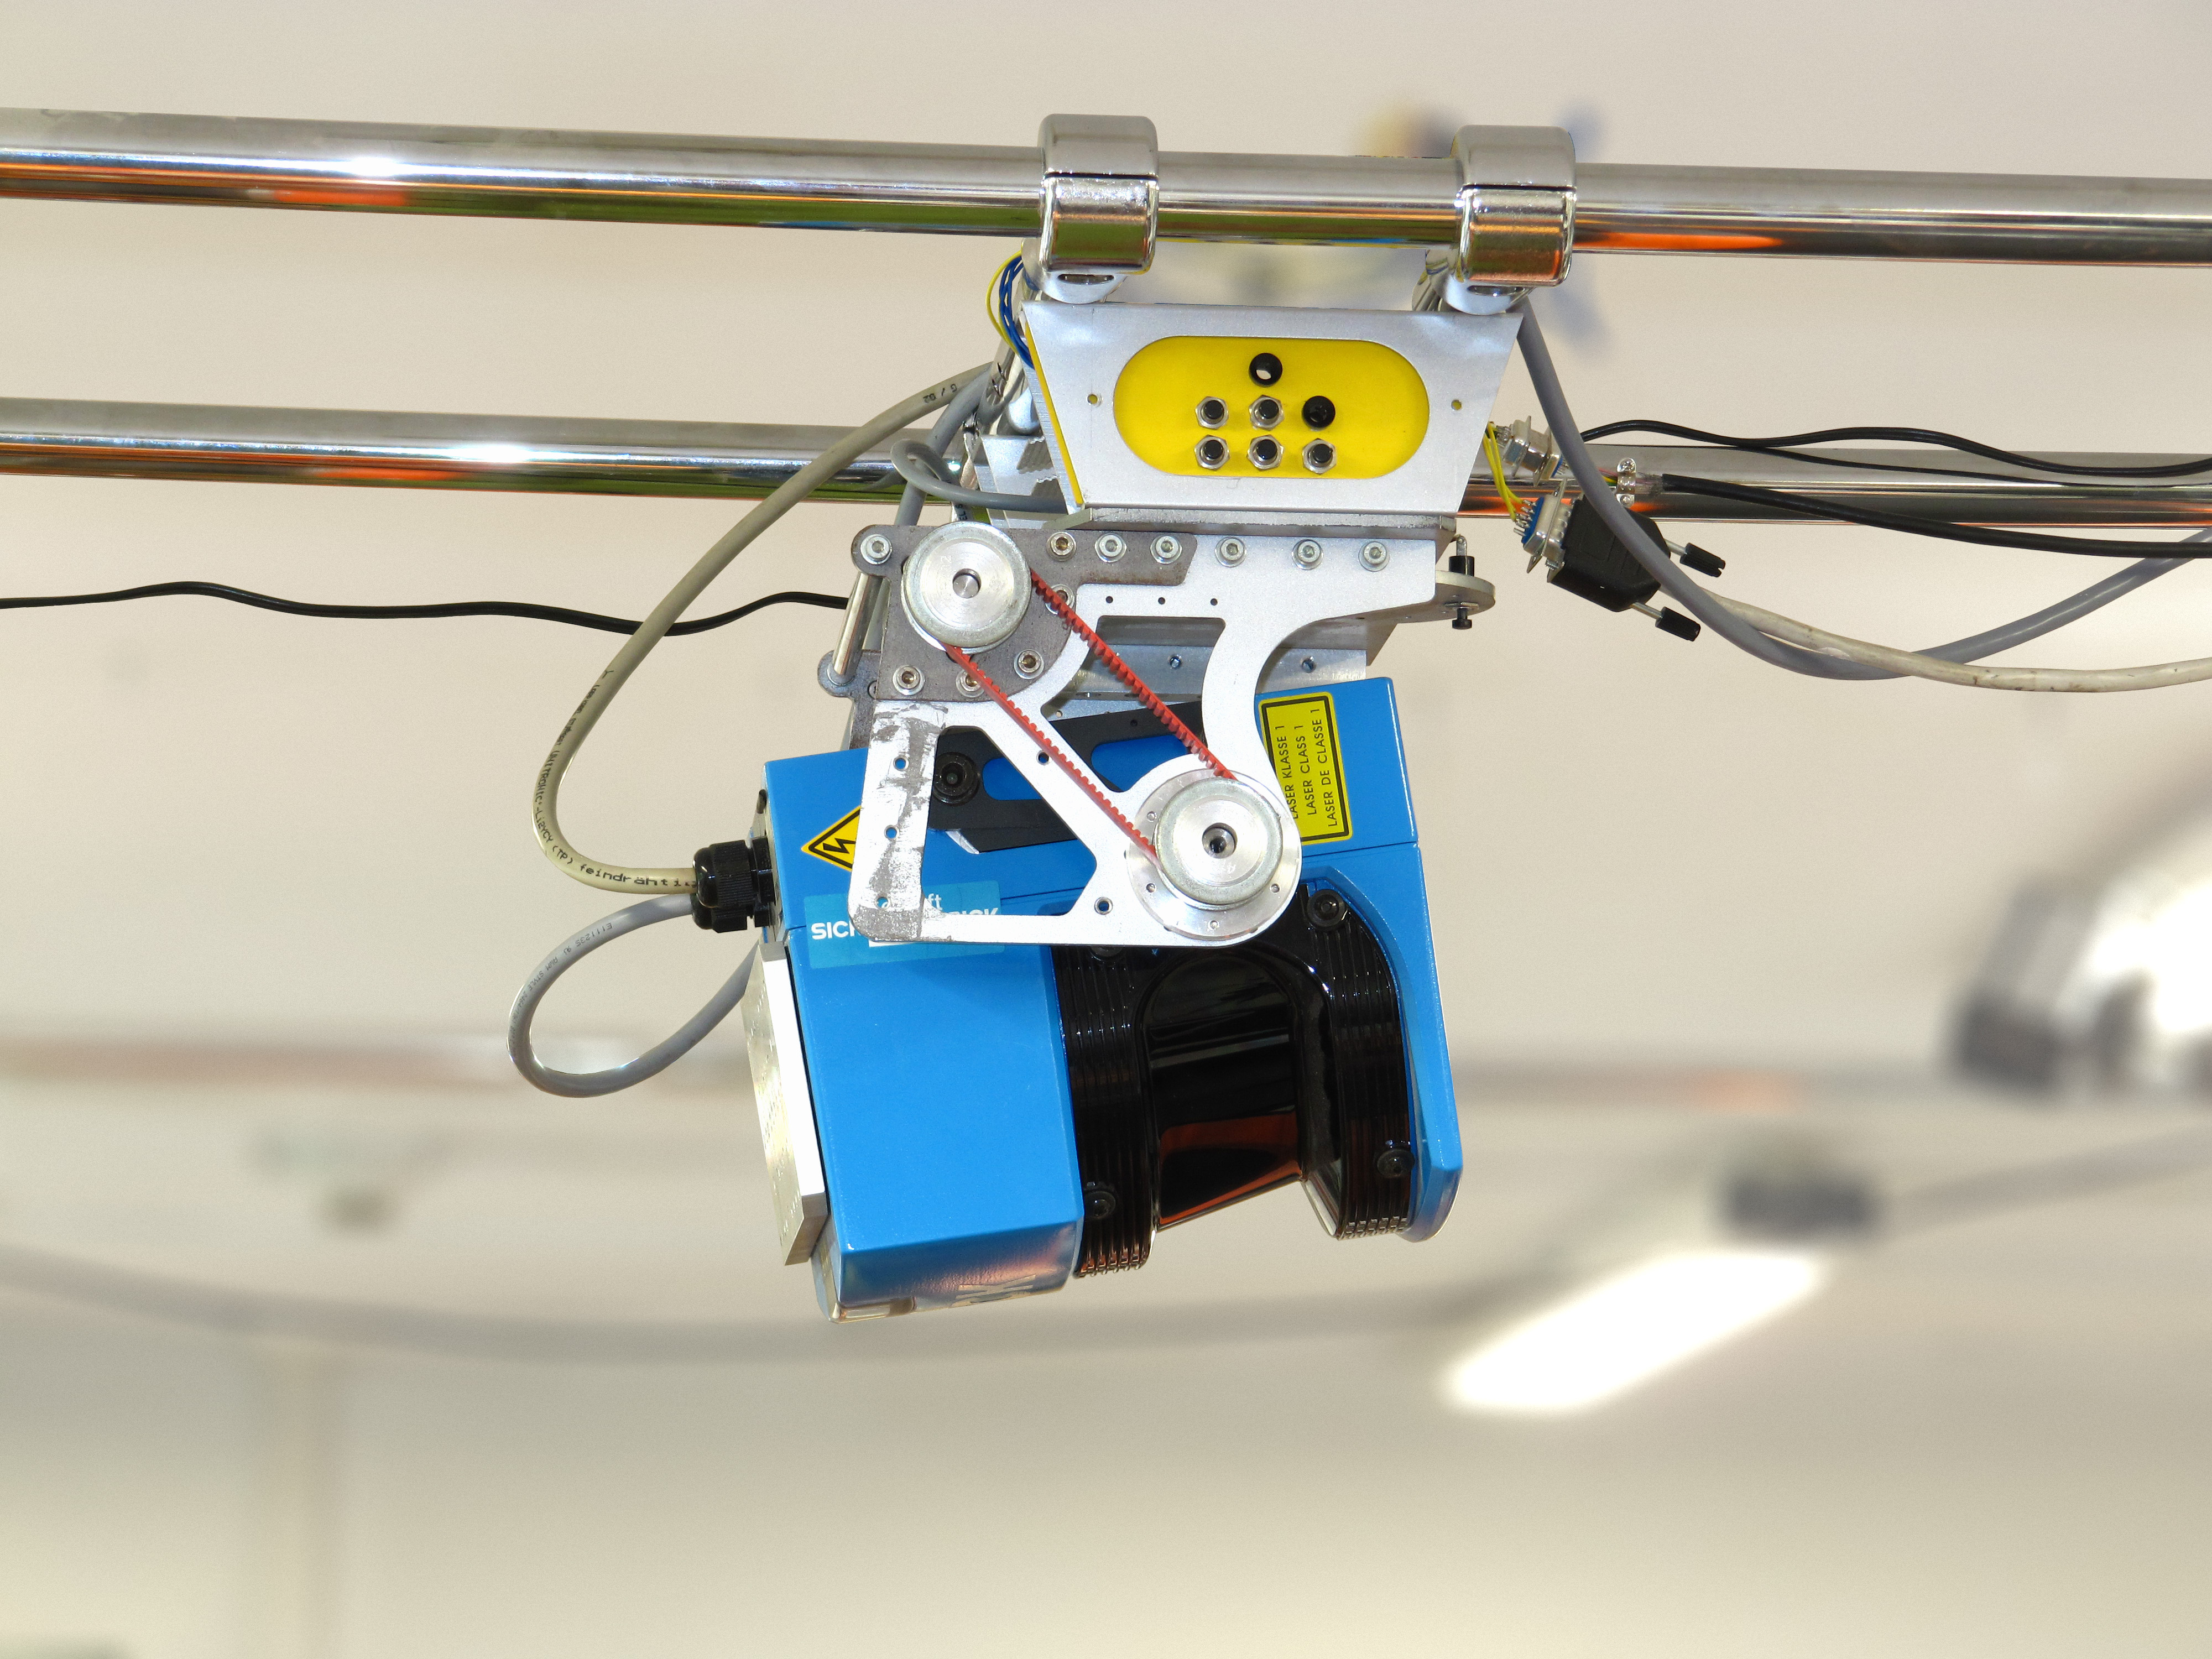
\includegraphics[height=6cm]{../../Common/img/sick_obrotnica} 
\caption{Skaner laserowy Sick LMS200 zamocowany na obrotnicy}
\label{fig:sick_obrotnica}
\end{figure}

\subsection{Sposoby interpolacji map głębi} 

Najprostszym sposobem wykorzystania uzyskiwanej informacji jest zapisanie
uzyskiwanych wyników wprost w mapie głębi. Można jednak wykorzystać fakt, że
skany wykonywane są w pewnych określonych sekwencjach, głównie liniami. Dzięki
temu w trakcie zbierania kolejnych pomiarów można dokonywać od razu
interpretacji i przetwarzania tych danych w celu stworzenia innej reprezentacji
otoczenia. W każdej kolejnej zeskanowanej linii można wyszukiwać za pomocą
odpowiednich algorytmów odcinki proste, a te zebrane w kolejnych skanach mogą
byc składane w większe płaszczyzny. Obliczenia te wykonywane są w tym samym
czasie, co zbieranie pomiarów, dzięki czemu praktycznie od razu po wykonaniu
ostatniego skanu dostajemy oprócz samej mapy głębi dodatkowe informacje o
geometrii sceny. Kolejne etapy opisanej agregacji danych
pokazane są na rysunku~\ref{fig:laser_aggregate}~\cite{Surmann01a3d}.

\begin{figure}[h!]
\centering
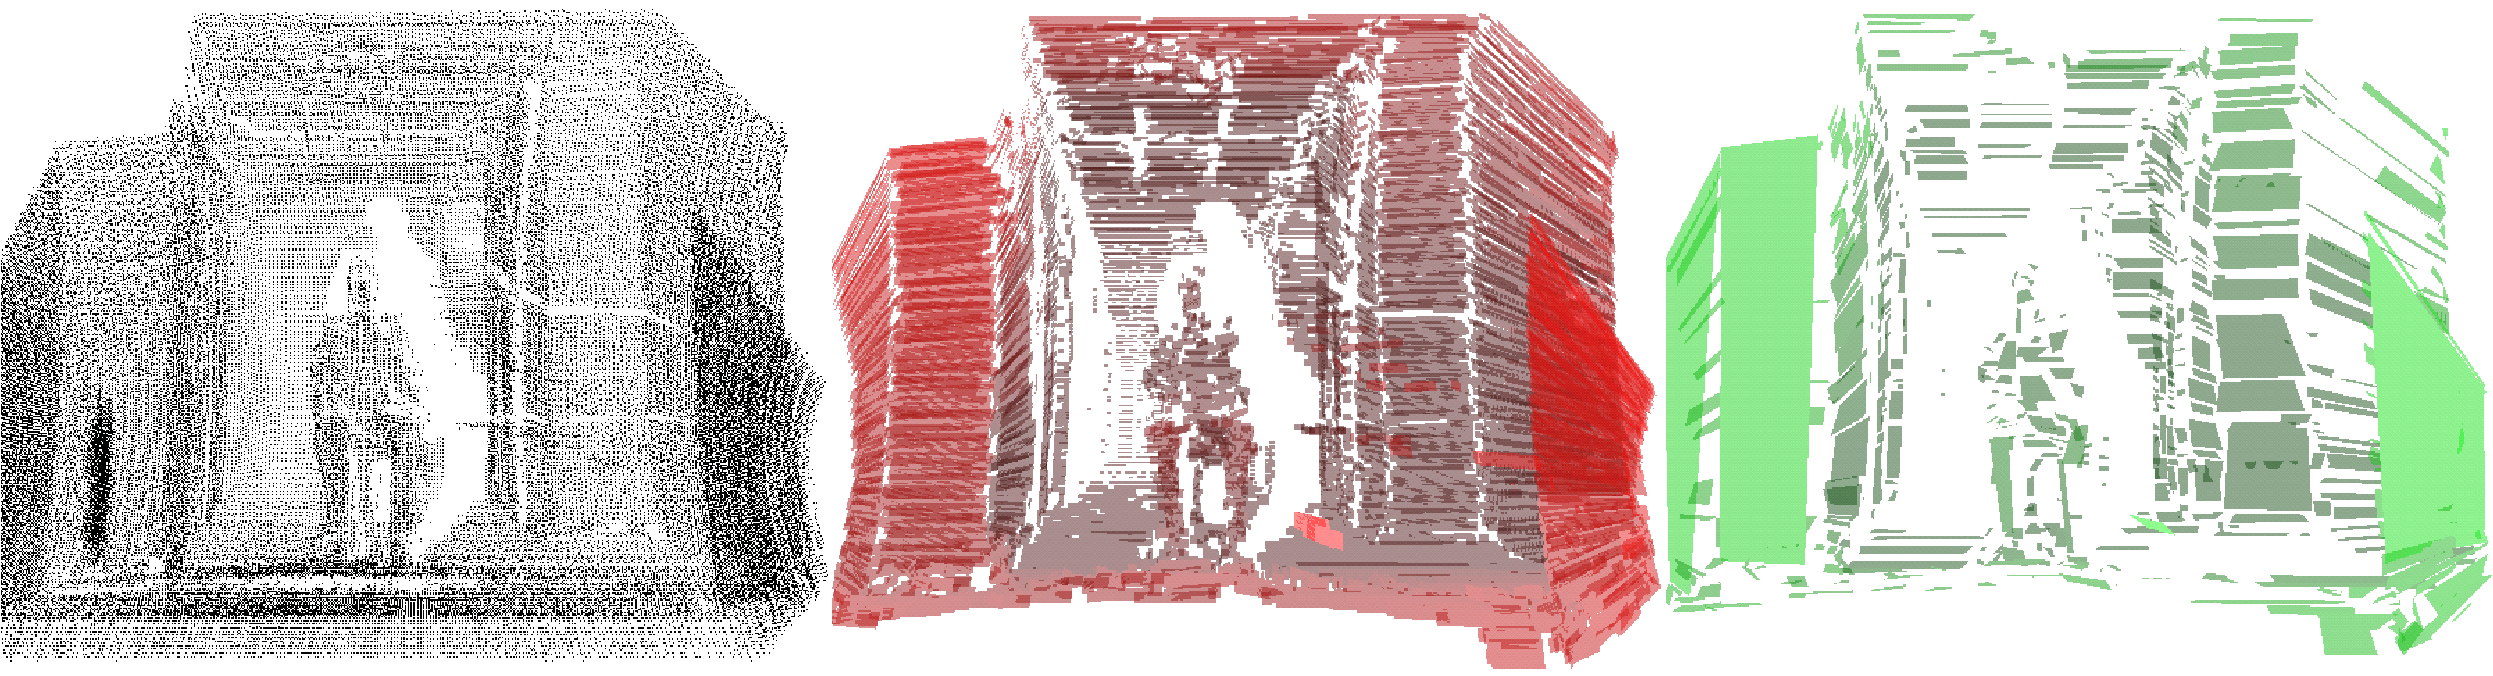
\includegraphics[width=12cm]{../../Common/img/laser_aggregate} 
\caption{Kolejne poziomy agregacji danych zebranych przy pomocy skanera
laserowego}
\label{fig:laser_aggregate}
\end{figure}

%%%%%%%%%%%%%%%%%%%%%%%%%%%%%%%%%%%%%%%%%%%%%%%%%%%%%%%%%%%%%%%%%%%%%%%%%%%%%%%%
%%%%%%%%%%%%%%%%%%%%%%%%%%%%%%%%%%%%%%%%%%%%%%%%%%%%%%%%%%%%%%%%%%%%%%%%%%%%%%%%
\section{Stereowizja}
%%%%%%%%%%%%%%%%%%%%%%%%%%%%%%%%%%%%%%%%%%%%%%%%%%%%%%%%%%%%%%%%%%%%%%%%%%%%%%%%
%%%%%%%%%%%%%%%%%%%%%%%%%%%%%%%%%%%%%%%%%%%%%%%%%%%%%%%%%%%%%%%%%%%%%%%%%%%%%%%%

%-------------------------------------------------------------------------------
\subsection{Zasada działania}
%-------------------------------------------------------------------------------

Stereowizja jest techniką obrazowania opierającą się na analizie obrazów wielu
(najczęściej dwóch) kamer. Algorytmy bazują na dysparacji, czyli względnej
odległości pomiędzy obrazami tego samego punktu w różnych kamerach, można w
nich wydzielić 3 kroki:

\begin{enumerate}
\item detekcja punktów charakterystycznych
\item dopasowanie odpowiedników
\item rekonstrukcja współrzędnych 3D
\end{enumerate}

Rysunek~\ref{fig:epipolar} przedstawia poglądowo zasadę działania algorytmów
stereowizyjnych. Rzeczywiste punkty $X$, $X_1$, $X_2$ oraz $X_3$ są współliniowe
względem lewej kamery (widoczne w obrazie jako ten sam punkt $X_L$). W obrazie z
prawej kamery punkty te są już rozróżnialne (punkt $X$ jest widoczny jako punkt
$X_R$). Znając współrzędne środków optycznych ($O_L$, $O_R$) i orientacje obu
kamer można wyznaczyć współrzędne linii epipolarnych dla badanych punktów, a
także rzeczywiste współrzędne tych punktów (na podstawie ich współrzędnych w
obu obrazach). W stereowizji najczęściej kamery ustawia się tak, aby ich osie
optyczne były możliwie równoległe, dzięki czemu łatwo wyznacza się linie
epipolarne (są poziome w obrazie) oraz odpowiednie punkty charakterystyczne.

\begin{figure}[h!]
\centering
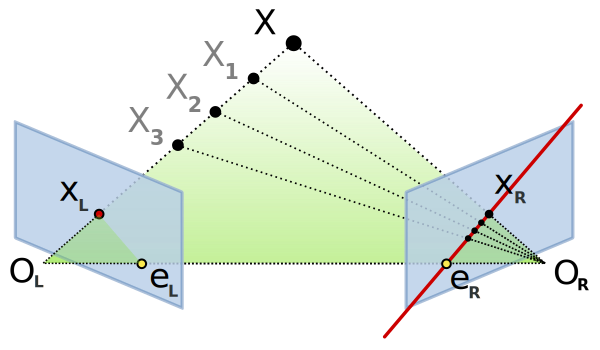
\includegraphics[width=8cm]{../../Common/img/Epipolar_geometry} 
\caption{Geometria dwubiegunowa}
\label{fig:epipolar}
\end{figure}

Dodatkowo konieczne jest wstępne przetworzenie obrazów tak, aby przedstawiały
one widok w taki sposób, jakby płaszczyzny obrazowania kamer były równoległe
(proces ten zwany jest rektyfikacją obrazu). W tym celu konieczna jest wstępna
kalibracja układu kamer, dająca w wyniku położenie kamer względem siebie
(przesunięcie oraz obrót), a także wyliczająca parametry wewnętrzne każdej z
kamer (zniekształcenia wnoszone przez soczewki obiektywu). Proces kalibracji
przeprowadza się raz dla danego położenia kamer, po każdorazowej zmianie ich
pozycji konieczna jest powtórna kalibracja. Rysunek~\ref{fig:stereo_steps}
przedstawia koleejne kroki podczas odtwarzania informacji o głębi z dwóch kamer.

\begin{figure}[h!]
\centering
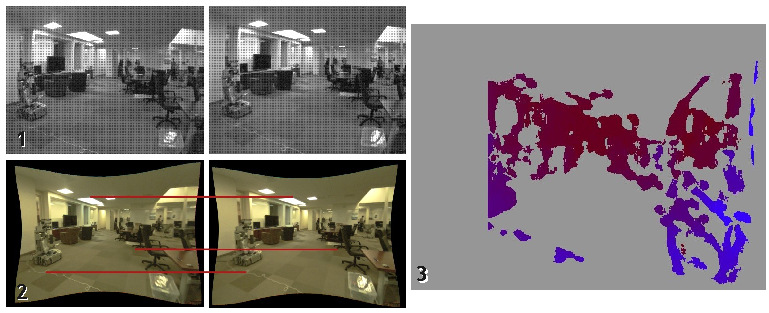
\includegraphics{../../Common/img/stereo_steps} 
\caption[Kolejne kroki podczas przetwarzania w stereowizji]
{Kolejne kroki podczas przetwarzania w stereowizji. 1: obraz pobrany
bezpośrednio z kamer; 2: obraz po interpolacji kolorów i rektyfikacji,
zaznaczone są także przykładowe, dopasowane punkty charakterystyczne; 3:
wynikowa mapa głebi dla podanej sceny.}
\label{fig:stereo_steps}
\end{figure}

%-------------------------------------------------------------------------------
\subsection{Wymagania sprzętowe}
%-------------------------------------------------------------------------------

Najważniejszym elementem przy stereowizji są kamery -- uzyskane rezultaty zależą
bezpośrednio od ich jakości. Stosowanie kamer z interfejsem analogowym jest
możliwe, jednak nie jest zalecane przy dynamicznych scenach. Obiekty
poruszające się z dużą szybkością są wykrywane błędnie bądź całkowicie
ignorowane ze względu na występujące rozmycie wynikające ze stosowania
przeplotu podczas akwizycji z kamer analogowych. Najlepsze wyniki uzyskuje się
stosując dobrej jakości kamery z interfejsami cyfrowymi, jednak ich koszt jest
dużo wyższy.

Samo rozmieszczenie kamer również ma istotny wpływ na uzyskiwane wyniki --
kamery umieszczone blisko siebie będą dawały dobre wyniki dla obiektów
znajdujących się blisko nich, kamery rozmieszczone szerzej pozwalają na
uzyskanie lepszej rozdzielczości dla obiektów znajdujących się daleko kosztem
częściowej bądź całkowitej utraty informacji o obiektach bliskich. Od
rozdzielczości kamery zależy uzyskiwana rozdzielczość przy rekonstrukcji sceny
3D, jednak wraz z jej wzrostem rośnie czas wymagany do przetworzenia
pojedynczej klatki obrazu.

\begin{figure}[h!]
\centering
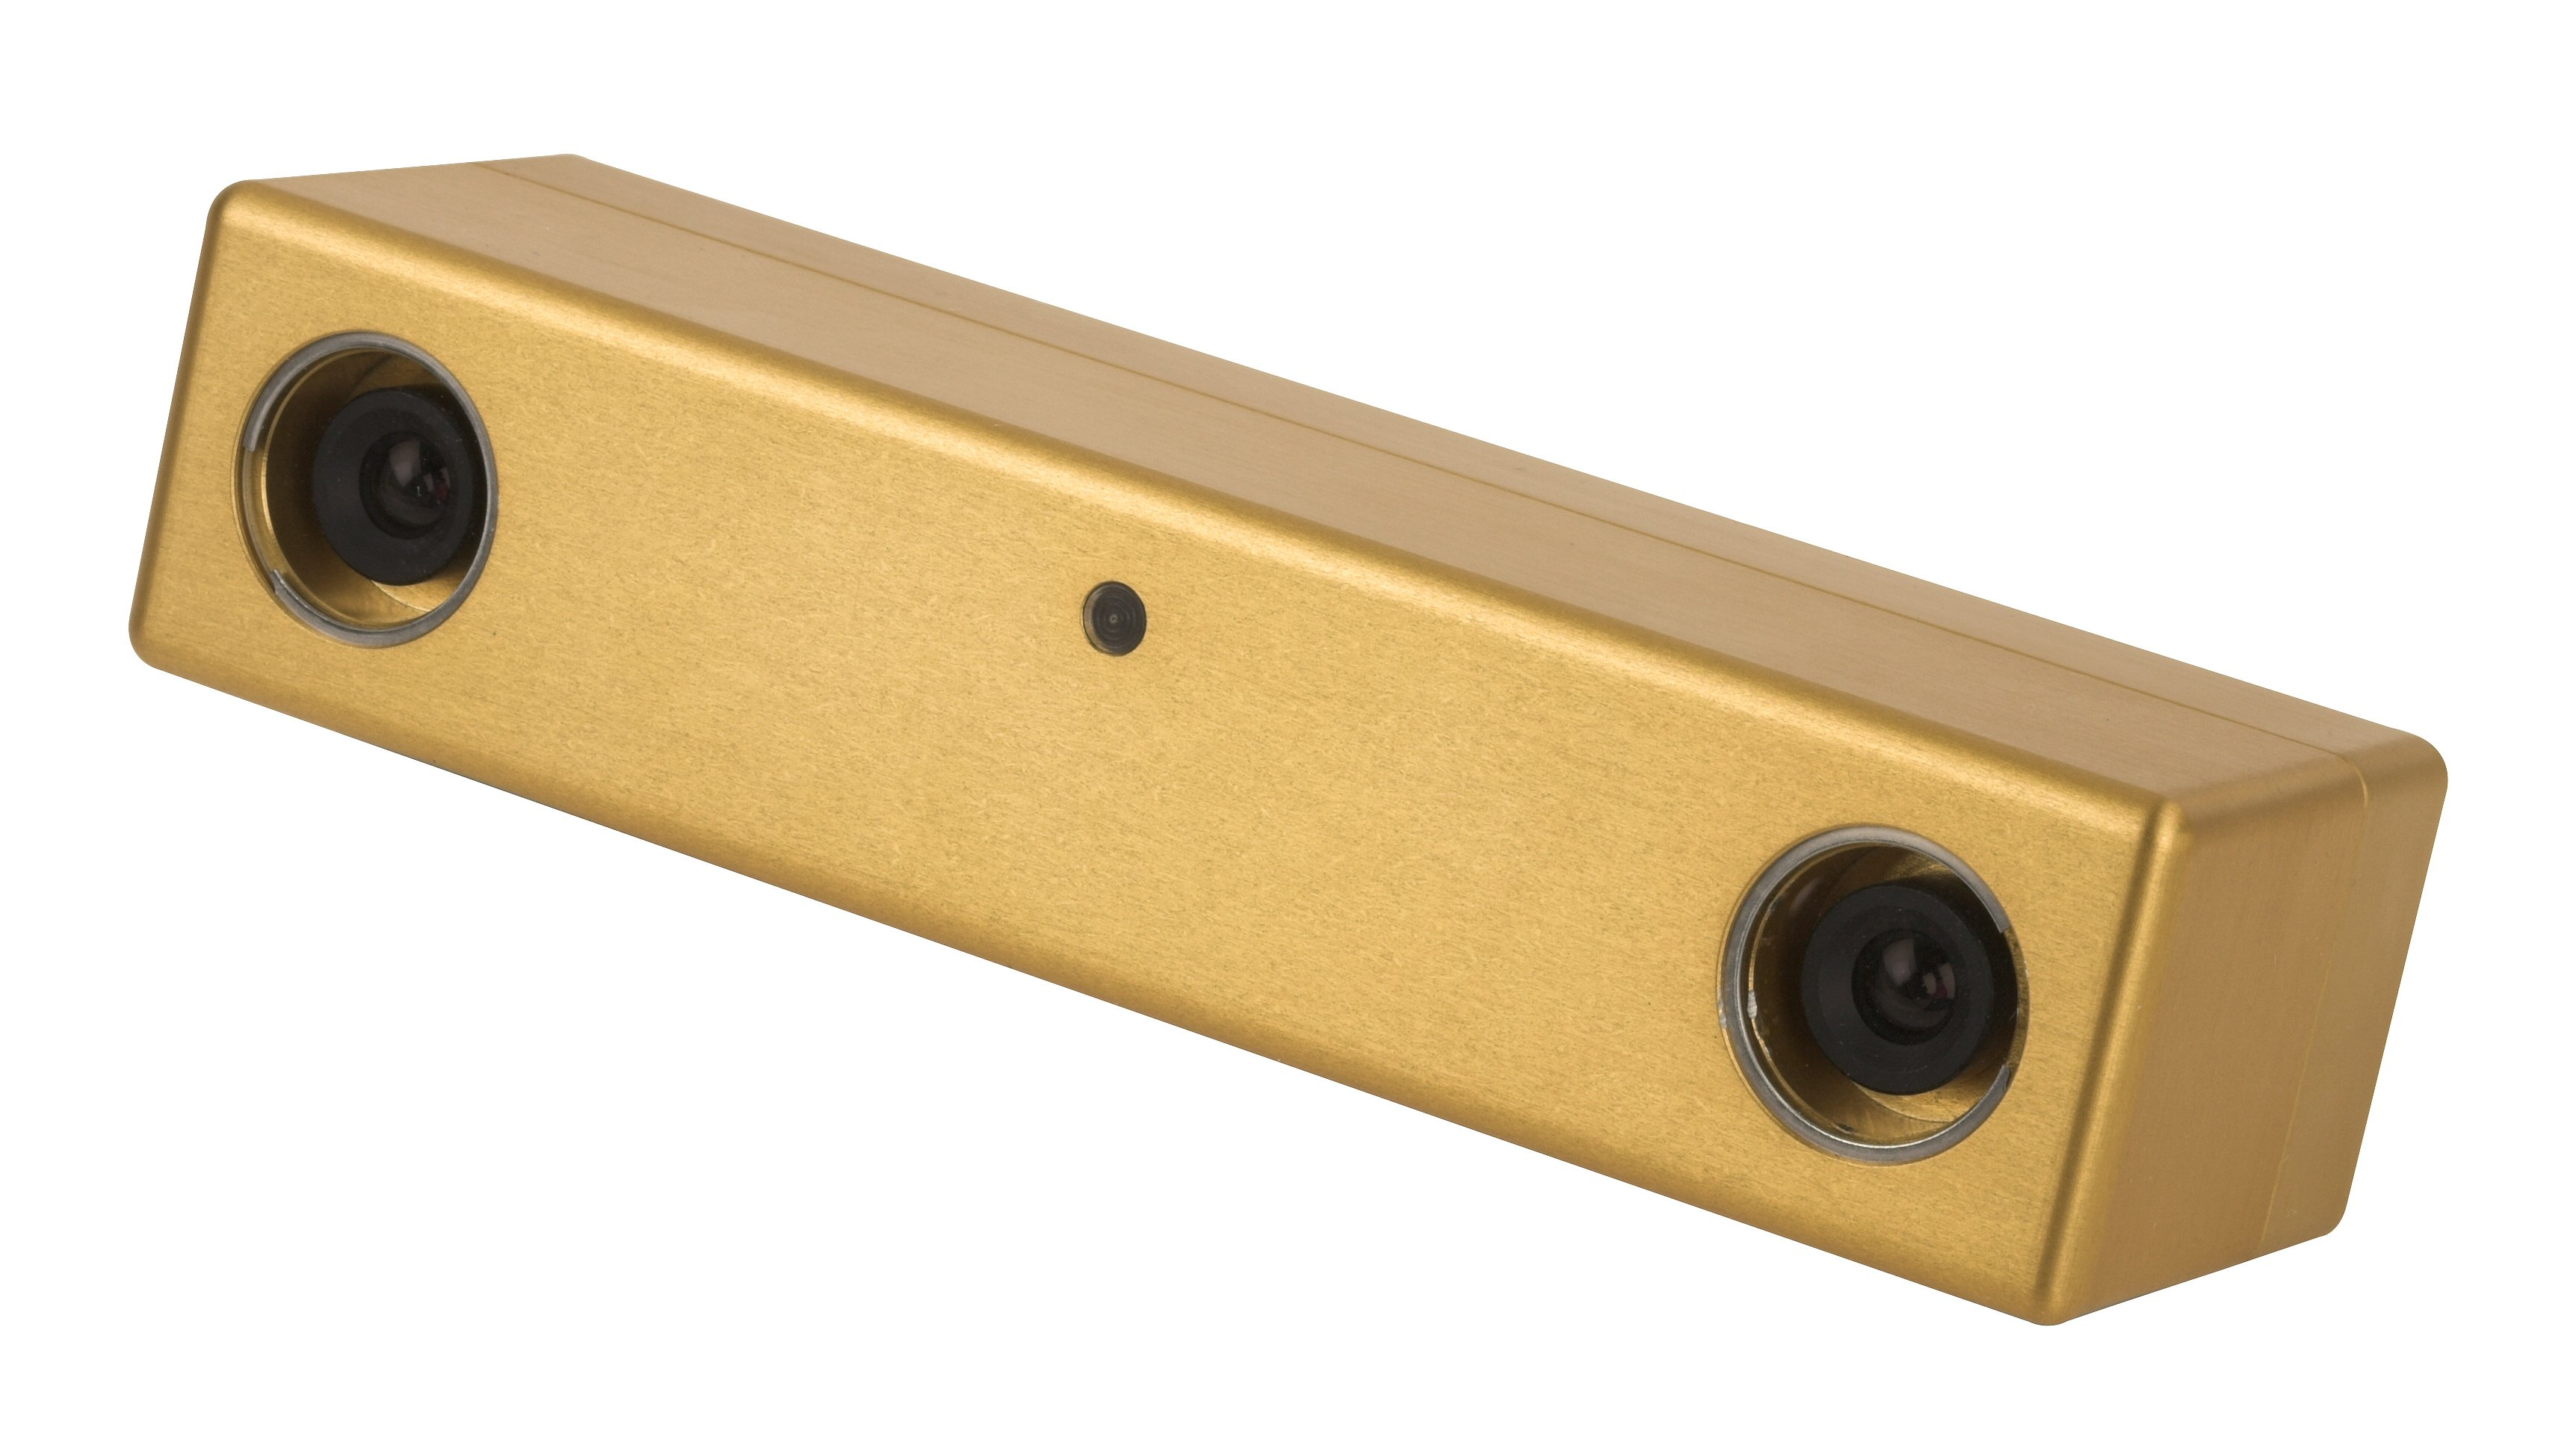
\includegraphics[width=8cm]{../../Common/img/bumblebee} 
\caption{Kamera do stereowizji Bumblebee X2}
\label{fig:bumblebee}
\end{figure}

Problemem może być samo mechaniczne mocowanie kamer. Musi być ono wykonane
bardzo solidnie, gdyż w przypadku nawet małej zmiany orientacji kamer względem
siebiewymagana jest ponowna kalibracja całego systemu. Aby pozbyć się tej wady
można stosować zintegrowane moduły zawierające dwie (bądź więcej) kamery w
jednej obudowie, to jednak uniemożliwia eksperymentowanie z odległością kamer
od siebie (patrz rysunek~\ref{fig:bumblebee}).

%-------------------------------------------------------------------------------
\subsection{Złożoność obliczeń}
%-------------------------------------------------------------------------------

% TODO: wstawić odwołania w odpowiednie miejsca
\cite{4670774} \cite{Hirschmuller:2008:SPS:1340087.1340245}

Przy wykorzystaniu programowej wersji algorytmów stereowizyjnych działających
na przeciętnym komputerze domowym, można osiągnąć wydajność od kilku do
kilkunastu klatek na sekundę. W związku z tym rozwiązania programowe słabo
nadają się do wykorzystania w środowisku, które ulega częstym i dynamicznym
zmianom (a takie jest otoczenie robota mobilnego).

Dużo lepiej sprawdzają się rozwiązania sprzętowe, w których algorytm tworzenia
mapy dysparacji zaimplementowany jest w układach FPGA zintegrowanych w jednym
module z kamerami. W tym przypadku wydajność jest stała i niezależna od platformy,
na której uruchomione będą algorytmy sterowania robota, i wynosi (w zależności
od producenta) od kilkunastu do ponad 30 FPS. Największą wadą takiego rozwiązania
jest jego koszt -- wynoszący od kilkuset do kilku tysięcy dolarów. Dla porównania
dwie kamery analogowe można kupić za ok. 200\$.

%-------------------------------------------------------------------------------
\subsection{Zastosowania}
%-------------------------------------------------------------------------------

Algorytm opiera się o wykrywanie punktów charakterystycznych w obrazie, a to
najczęściej sprowadza się do analizy obrazu krawędziowego. W związku z tym
obiekty o jednolitej, drobnej teksturze (bądź całkowicie gładkie) są słabo bądź
całkowicie niewykrywalne. W najlepszym wypadku wykrywane są jedynie ich
krawędzie, co prowadzi do powstawania dużych, niezidentyfikowanych obszarów w
obrazie (rysunek~\ref{fig:stereo_3} przedstawia taką sytuację).

Jednym z rozwiązań tego problemu może być zastosowanie dodatkowego projektora
wyświetlającego specjalnie przygotowany wzór (przykład na
rysunku~\ref{fig:stereo_texture}) w celu pokrycia obiektów sztuczną teksturą
umożliwiającą poprawę wyników stereowizji. Drugą możlwością poprawy sytuacji
jest stosowanie dodatkowego etapu przetwarzania obrazu po wygenerowaniu
wstępnej mapy głębokości. Po segmentacji obrazu na podstawie koloru wybierane
są obszary jednolite, a następnie w mapie głębi wypełniane są interpolowanymi
wartościami z ich krawędzi.

\begin{figure}[htpb!]
\centering
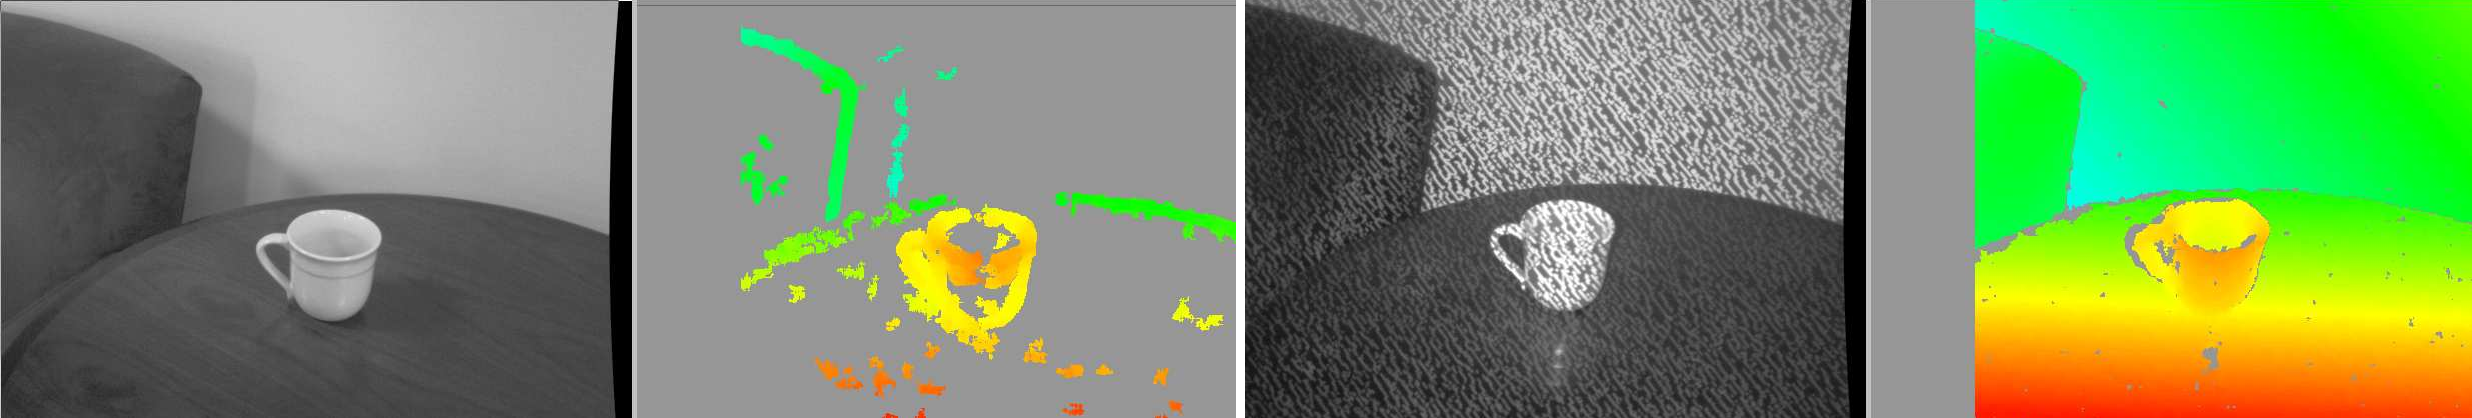
\includegraphics[width=16cm]{../../Common/img/stereo_texture} 
\caption[Przykład projekcji tekstury w celu poprawy jakości
stereowizji]{Przykład projekcji tekstury w celu poprawy jakości stereowizji
\cite{konolige-icra-2010-a} W kolejności od lewej: scena bez dodatkowego
oświetlenia, wygenerowana mapa głębi, scena z rzutowaną teksturą, poprawiona
mapa głębi}
\label{fig:stereo_texture}
\end{figure}

Oba rozwiązania dają dobre rezultaty, jednak komplikują bądź budowę urządzenia,
bądź wprowadzają dodatkowy narzut obliczeniowy. Projekcja tekstury bywa
z powodzeniem wykorzystywana w robotach mobilnych \cite{piorkowski2008}, a
bardziej skomplikowane algorytmy stosowane są na dużych robotach
manipulacyjno-przemysłowych, które są wyposażone w odpowiednio wydajne
jednostki obliczeniowe (np. robot PR2). Natomiast w robotach poruszających się
w naturalnym środowisku, gdzie występuje bardzo dużo szczegółów (a więc i
punktów charakterystycznych) stereowizja stosowana jest praktycznie bez żadnych
dodatkowych usprawnień i sprawdza się znakomicie (zwracane mapy głębi są
wypełnione w ponad 80\%, a algorytm działa w tempie powyżej 10FPS)
\cite{outdoor-stereo}.


%%%%%%%%%%%%%%%%%%%%%%%%%%%%%%%%%%%%%%%%%%%%%%%%%%%%%%%%%%%%%%%%%%%%%%%%%%%%%%%%
%%%%%%%%%%%%%%%%%%%%%%%%%%%%%%%%%%%%%%%%%%%%%%%%%%%%%%%%%%%%%%%%%%%%%%%%%%%%%%%%
\section{Światło strukturalne}
%%%%%%%%%%%%%%%%%%%%%%%%%%%%%%%%%%%%%%%%%%%%%%%%%%%%%%%%%%%%%%%%%%%%%%%%%%%%%%%%
%%%%%%%%%%%%%%%%%%%%%%%%%%%%%%%%%%%%%%%%%%%%%%%%%%%%%%%%%%%%%%%%%%%%%%%%%%%%%%%%

%-------------------------------------------------------------------------------
\subsection{Zasada działania}
%-------------------------------------------------------------------------------

Inną metodą pomiaru i odtwarzania informacji i głębi sceny bazującą na analizie
obrazu jest wykorzystanie światła strukturalnego. Na scenę rzucane jest światło
formujące znany wzór, a kamera umieszczona jest w taki sposób, aby obserwować
scenę pod innym kątem niż orientacja rzutnika. Na podstawie odczytanej deformacji
wzorca prz użyciu algorytmów bazujących na riangulacji wyliczane są rzeczywiste
współrzędne punktów w obrazie. 

\begin{figure}[htb!]
\centering
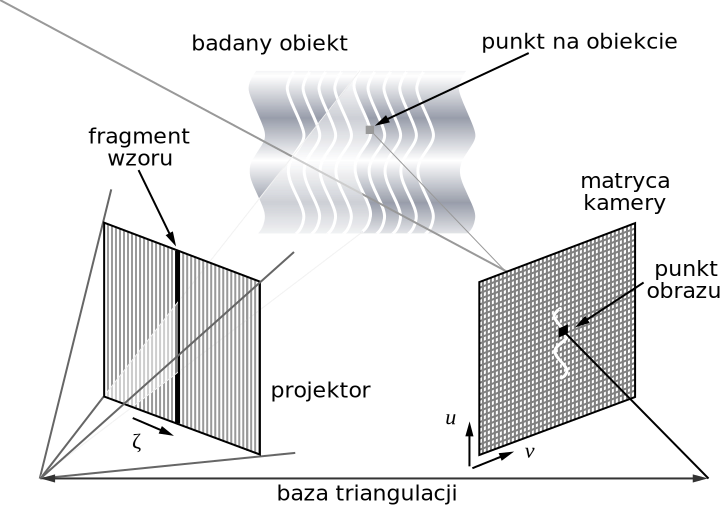
\includegraphics[width=10cm]{../../Common/img/struct} 
\caption[Schemat działania skanera opartego o światło strukturalne]
{Schemat działania skanera opartego o światło strukturalne. Na podstawie:
http://en.wikipedia.org/wiki/File:1-stripesx7.svg}
\label{fig:struct_principle}
\end{figure}

Rzutowane mogą być różne wzory, zaczynając od pojedynczego punktu, przez
wzory złożone z linii (statycznych bądź przesuwających się po
scenie, w takim przypadku scena jest analizowana stopniowo), aż po złożone,
pseudoloswe wzory (także kolorowe) oraz sekwencje wzorów \cite{1588327}. W
przypadku korzystania z sekwencji wzorów wymagany jest statyczny charakter
sceny, sceny dynamiczne wymagają stosowania pojedynczych, skomplikowanych
struktur.

\begin{figure}[h!]
\centering
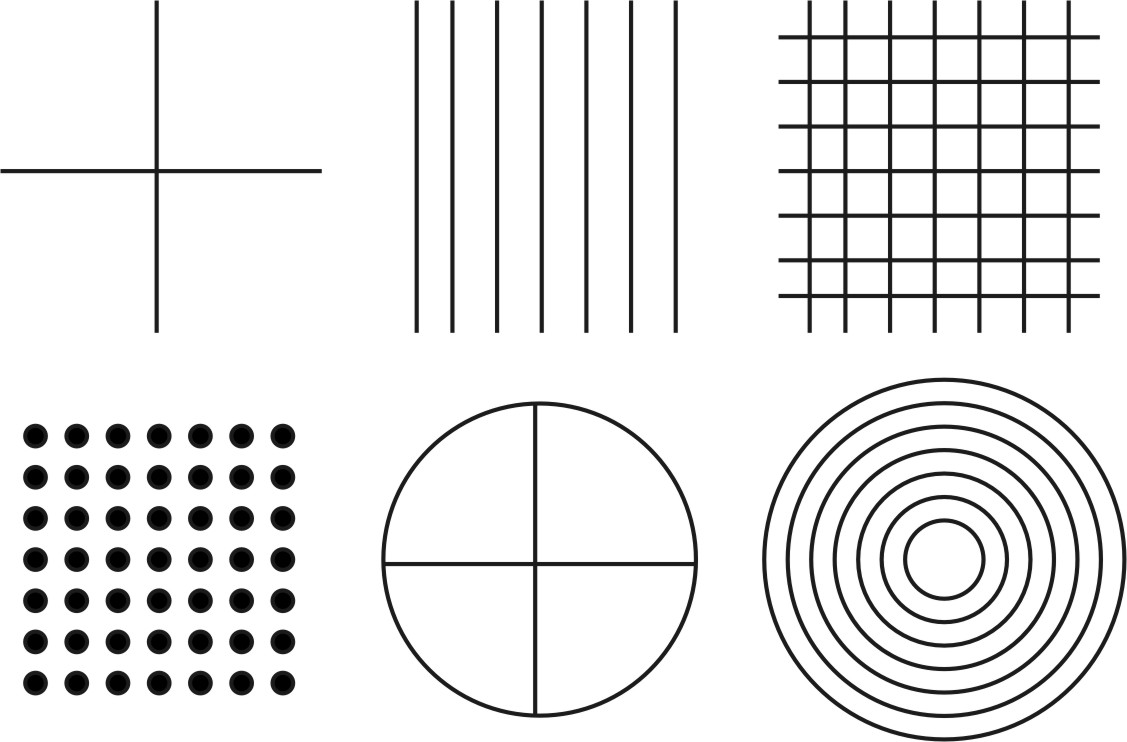
\includegraphics[width=8cm]{../../Common/img/struct_patterns} 
\caption[Wzorce wykorzystywane przy obrazowaniu światłem strukturalnym]
{Wzorce wykorzystywane przy obrazowaniu światłem strukturalnym}
\label{fig:struct_patterns}
\end{figure}

%-------------------------------------------------------------------------------
\subsection{Zastosowania}
%-------------------------------------------------------------------------------

Głównym kryterium przy wyborze konkretnej realizacji skanera opartego o światło
strukturalne jest charakter analizowanej sceny. W przypadku skanowania obiektów
statycznych (np. podczas automatycznego tworzenia modeli trójwymiarowych)
możliwe jest zastosowanie sekwencji wzorców, np. kodu Graya. Stosowane są też
różne rozwiązania pomocnicze w celu zeskanowania obiektu ze wszystkich stron bez
jego obracania (np. zestaw specjalnie ustawionych luster) \cite{LanmanCT07}.

\begin{figure}[!ht]
\centering
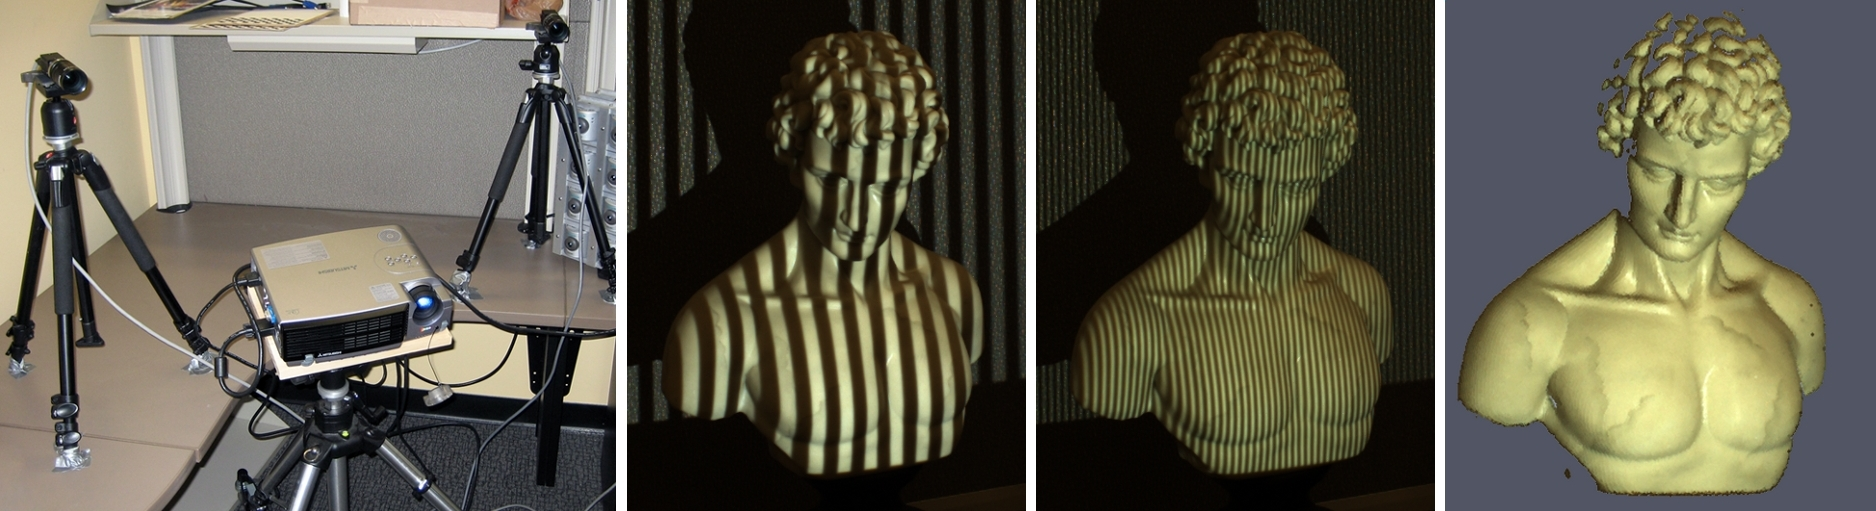
\includegraphics[width=14cm]{../../Common/img/struct_all} 
\caption[Przykład wykorzystania światła strukturalnego do modelowania obiektów]
{Przykład wykorzystania światła strukturalnego do modelowania obiektów. Na
pierwszym zdjęciu widać układ pomiarowy, następnie dwa wybrane etapy oświetlania
kodem Graya oraz wynikowy model otrzymany po oświetleniu 40-toma wzorcami.
Źródło: http://web.media.mit.edu/~dlanman/}
\label{fig:struct_all}
\end{figure}

Do zastosowań czasu rzeczywistego, jak już wspomniano wcześniej, nadają się
jedynie wzorce pojedyncze. Dzięki temu każda otrzymana klatka obrazu zawiera
informacje o całym modelu, w metodach opartych o wzorce sekwencyjne obiekt
przesuwający się pomiędzy kolejnymi naświetleniami powoduje zakłamanie wyników. 
Wśród takich metod wyróżnić można oparte o wzorce kodowane geometrycznie i
kolorowo. Pierwsza z metod wykorzystuje jednobarwne wzorce geometryczne
zakodowane w taki sposób, aby poszczególne jego bloki były unikalne w pewnym
otoczeniu. W przypadku tej drugiej metody stosowane są np. różnokolorowe pasy
bądź szachownice, a z układu kolorów rekonstruowana jest powierzchnia obiektów.
Rozwiązania te cechują się dużą szybkością działania, od kilkunastu do ponad
stu klatek przetwarzanych w ciągu sekundy \cite{4429304}.

\begin{figure}[h!]
\centering
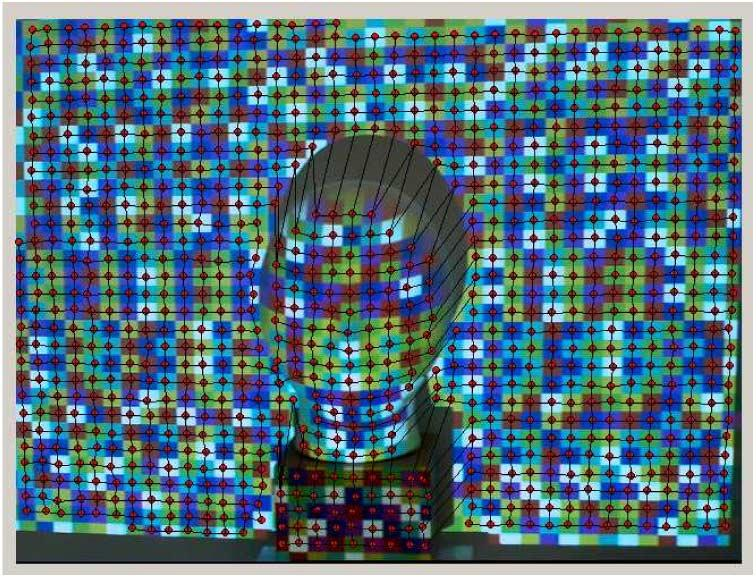
\includegraphics[width=8cm]{../../Common/img/struct_color} 
\caption[Wzorzec kodowany kolorem]
{Jedna z możliwości kolorowego kodowania wzorców \cite{4429304}}
\label{fig:struct_color}
\end{figure}

W zastosowaniach robotycznych, w przypadku, kiedy maszyny mają działać we
wspólnym otoczeniu z ludźmi, wzorce kodowane kolorami są niewygodne -- musza one
działać w paśmie światła widzialnego, co może przeszkadzać będącym w pobliżu
ludziom. W takim wypadkuz zdecydowanie lepiej sprawdzają się wzorce
geometryczne, których rzutniki mogą działać w podczerwieni, a więc w sposób
niewidoczny i nieprzeszkadzający użytkownikom. W taki właśnie sposób działa
Microsoft Kinect, opisany dokładnie w rozdziale~\ref{chap:sprzet}.  

Największą niedogodnością związaną z wykorzystaniem obrazowania opartego o
rzutowanie wzorców jest konieczność dokładnego wykrycia tego wzoru. Dlatego też
najczęściej stosowane jest ono na niewielkie odległości, przy skanowaniu
pojedynczych obiektów. Przy stosowaniu na większe odległości konieczne jest
stosowanie bądź projekcji w paśmie podczerwonym (aby wykluczyć zakłócenia od
tradycyjnych źródeł światła), bądź wykorzystanie projektorów o bardzo dużej
mocy. Żaden z wariantów nie sprawdza się jednak na otwartej przestrzeni, gdzie
światło słoneczne zakłóca działanie praktycznie wszystkich sensorów tego typu.

%-------------------------------------------------------------------------------
\subsection{Rozwiązania programowe i sprzętowe} 
%-------------------------------------------------------------------------------

W przypadku stosowania algorytmów zaimplementowanych programowo uruchamianych na
komputerze sterującym można wymienić praktycznie takie same wady, jak przy
stereowizji, Największą z nich jest obciążenie systemu, gdyż algorytm jest
dość skomplikowany. Rozwiązania sprzętowe rozwiązują problem szybkości działania
i obciążenia komputera sterującego, jednak ich cena przez bardzo długi czas
była wysoka (rzędu setek do tysięcy dolarów). Pod koniec 2010 roku pojawił się
na runku wspomniany wcześniej Microsoft Kinect -- urządzenie o cenie o
rząd wielkości niższej, będące faktycznie sprzętowym sensorem głębi opartym o
analizę światła strukturalnego. Niską cenę zawdzięcza masowej produkcji -- jest
produkowany jako kontroler do gier, i jako taki ma zdecydowanie większy rynek
zbytu niż tradycyjne, specjalizowane rozwiązania. 

Przed pojawieniem się na rynku urządzenia Microsoft Kinect, w robotyce mobilnej
stosowane były głównie rozwiązania oparte o obrazowanie na podstawie projekcji
pojedynczych linii (\cite{120445,5246792}), głównie ze względu na prostotę
koniecznych obliczeń i szybkość działania całego systemu. 


%%%%%%%%%%%%%%%%%%%%%%%%%%%%%%%%%%%%%%%%%%%%%%%%%%%%%%%%%%%%%%%%%%%%%%%%%%%%%%%%
%%%%%%%%%%%%%%%%%%%%%%%%%%%%%%%%%%%%%%%%%%%%%%%%%%%%%%%%%%%%%%%%%%%%%%%%%%%%%%%%
\section{Pomiar czasu przelotu wiązki światła}
%%%%%%%%%%%%%%%%%%%%%%%%%%%%%%%%%%%%%%%%%%%%%%%%%%%%%%%%%%%%%%%%%%%%%%%%%%%%%%%%
%%%%%%%%%%%%%%%%%%%%%%%%%%%%%%%%%%%%%%%%%%%%%%%%%%%%%%%%%%%%%%%%%%%%%%%%%%%%%%%%

Kamery TOF\footnote{z ang. {\it time-of-flight}, czas przelotu} działają na zasadzie
pomiaru czasu przelotu wiązki światła od projektora do kamery po jego odbiciu od
obiektów. Działanie to jest analogiczne do działania skanerów laserowych, z tą różnicą,
że w przypadku skanerów emitowana jest pojedyncza wiązka światła, natomiast kamery TOF
oświetlają i wykonują pomiar całej sceny naraz.

%-------------------------------------------------------------------------------
\subsection{Zasada działania i wykorzystanie}
%-------------------------------------------------------------------------------

Kamery TOF mogą działać w oparciu o dwie główne metody: bezpośredni pomiar
czasu przelotu wiązki światła (od błysku naświetlającego scenę do jego
zarejestrowania na matrycy) bądź pośredni pomiar tej wielkości z różnicy fazy
emitowanego światła (w tym przypadku bez przerwy emitowane jest modulowane
światło~\cite{910448}). W obu wypadkach wyliczony czas przelotu dla każdego
punktu zarejestrowanego obrazu jest proporcjonalny do jego odległości od kamery.

\begin{figure}[h!]
\centering
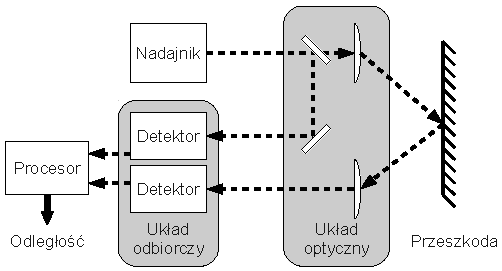
\includegraphics[width=8cm]{../../Common/img/tof} 
\caption{Schemat działania kamer TOF mierzących bezpośrednio czas przelotu}
\label{fig:tof}
\end{figure}

Kamery typu TOF są wykorzystywane w robotyce mobilnej głównie w robotach
operujących w pomieszczeniach~\cite{Prusak:2008:PEM:1462089.1462102}. Dokładność
uzyskiwanych pomiarów, szybkość działania i niskie obciążenie komputera
sterującego pozwalają na wykorzystanie otrzymywanego obrazu nie tylko do
wykrywania i omijania przeszkód, ale także do budowy mapy otoczenia i
samolokalizacji robota (na podstawie obserwacji punktów charakterystycznych w
mapie głębi). Sama technologia wykonania sensora sprawia jednak, że do
rejestracji obrazu kolorowego wymagana jest dodatkowa kamera, skalibrowana z
modułem głębi (niedogodność ta nie wystepuje przy stosowaniu stereowizji oraz
wielu metod opartych o analizę światła strukturalnego).

%-------------------------------------------------------------------------------
\subsection{Właściwości metody}
%-------------------------------------------------------------------------------

Zastosowanie metody opartej o pomiar czasu powrotu wiązki światła pozwala na
umieszczenie projektora i matrycy rejestrującej obraz bardzo blisko siebie (w
szczególności współosiowo, z diodami projektora umieszczonymi dookoła obiektywu
kamery), dzięki czemu nie występuje największa wada systemów opartych o
triangulację (stereowizja i światło strukturalne), czyli powstawanie cieni.
Spośród innych zalet tej metody pomiaru wymienić można chociażby zwartą
konstrukcję sensora (cały system składa się z pojedynczego modułu zawierającego
zarówno kamerę jak i oświetlacz), dzięki czemu jest on bardzo łatwy do
zastosowania w gotowym robocie. Nie bez znaczenia jest też szybkość działania --
dzięki naświetlaniu całej klatki jednocześnie oraz biorąc pod uwagę prędkość 
światła, możliwe jest uzyskanie prędkości nawet 100 klatek na sekundę, a dzięki
całkowicie sprzętowemu przetwarzaniu danych uzyskuje się bardzo niskie
obciążenie systemu -- kamera zwraca obraz zawierający bądź czas przelotu
światła, z którego w prosty sposób obliczyć można odległość, bądź od razu gotową
mapę głębi. Widać tutaj dużą przewagę nad innymi rozwiązaniami, gdzie wymagane
jest stosowanie skomplikowanych algorytmów w celu wyliczenia ostatecznej
odległości do obiektów.

\begin{figure}[h!]
\centering
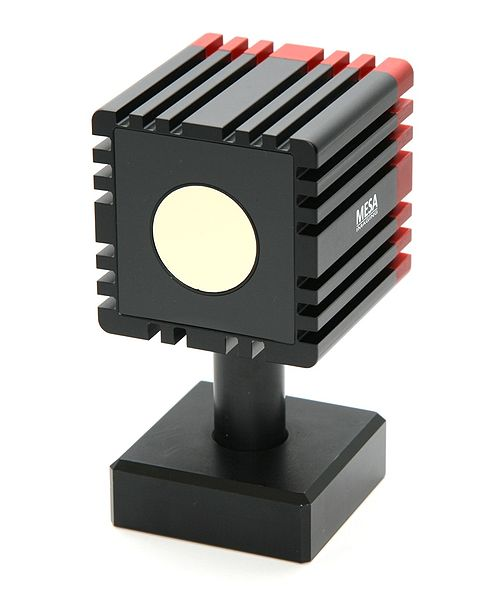
\includegraphics[height=5cm]{../../Common/img/sr4000} 
\caption[Kamera TOF SwissRanger SR4000]{Kamera TOF SwissRanger SR4000.
Rozdzielczość obrazu: 176x144px przy 54FPS, cena ok. 9000\$}
\label{fig:sr4000}
\end{figure}
 
Własności te sprawiają, że kamery TOF wydają się być bardzo dobrym rozwiązaniem
do zastosowania przy nawigacji robota. Niestety, mają też kilka wad, które to
wykorzystanie utrudniają. Pierwszą z nich jest cena -- jako że rozwiązania te są
stosunkowo nowe a także bardzo skomplikowane pod względem technicznym, ich cena
jest wielokrotnie wyższa od układów opartych na stereowizji lub świetle
strukturalnym. W porównaniu do tych metod niższa jest także rozdzielczość
uzyskiwanej mapy głębi -- obecnie produkowane sensory posiadają rozdzielczość
maksymalną rzędu 320x240px, a tańsze modele często posiadają rozdzielczość 
poniżej 100x100px. Sama technika wykonywania pomiaru ma kilka cech, które mogą
utrudniać jej wykorzystanie, np. występowanie wielokrotnych odbić, przez co
do sensora może dotrzeć i zostać zarejestrowane światło odbite i załamane od
obiektów znajdujących się bliżej, niż faktyczny punkt widziany w danym miejscu
matrycy. Podobnie zafałszowane pomiary mogą wystąpić przy obecności w
obserwowanej scenie silnych źródeł światła, praktycznie niemożliwe jest także
stosowanie tych metod w słoneczny dzień w terenie otwartym. Przy stosowaniu
wielu kamer TOF jednocześnie należy uwzględnić problem interferencji emitowanego
światła -- najczęściej rozwiązywany przez sekwencyjne odczyty z kolejnych kamer
(co z kolei zmniejsza faktyczną szybkość akwizycji danych).

\begin{figure}[h!]
\centering
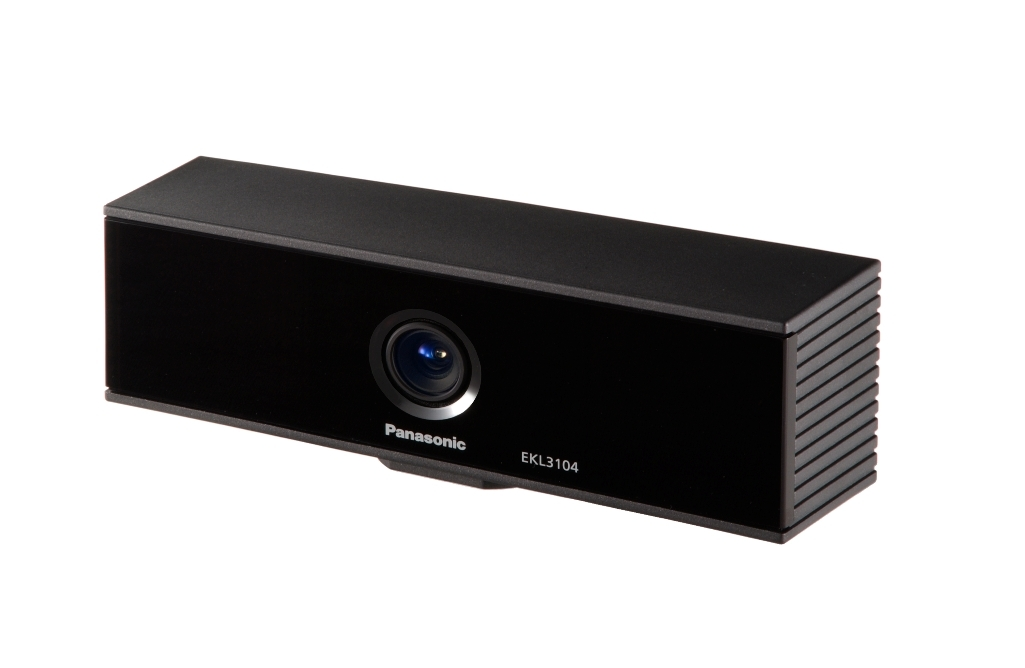
\includegraphics[height=5cm]{../../Common/img/dimager} 
\caption[Kamera TOF Panasonic D-IMager]{Kamera TOF Panasonic D-IMager.
Rozdzielczość obrazu: 160x120px przy 20FPS, cena ok. 3000\$}
\label{fig:dimager}
\end{figure}

%%%%%%%%%%%%%%%%%%%%%%%%%%%%%%%%%%%%%%%%%%%%%%%%%%%%%%%%%%%%%%%%%%%%%%%%%%%%%%%%
%%%%%%%%%%%%%%%%%%%%%%%%%%%%%%%%%%%%%%%%%%%%%%%%%%%%%%%%%%%%%%%%%%%%%%%%%%%%%%%%
\section{Porównanie dostępnych rozwiązań}
%%%%%%%%%%%%%%%%%%%%%%%%%%%%%%%%%%%%%%%%%%%%%%%%%%%%%%%%%%%%%%%%%%%%%%%%%%%%%%%%
%%%%%%%%%%%%%%%%%%%%%%%%%%%%%%%%%%%%%%%%%%%%%%%%%%%%%%%%%%%%%%%%%%%%%%%%%%%%%%%%

Ta część ma na celu porównanie dwóch dostępnych dla autora pracy rozwiązań --
stereowizji dwukamerowej i światła strukturalnego (sensora Microsoft Kinect).
Celem testów jest porównanie szybkości działania, obciążenia systemu i pokrycia
mapy głębi. Dokładność odwzorowania mapy głębi nie była obiektem testów, dlatego
wygenerowane mapy głębi mają różniące się skale kolorystyczne.

%-------------------------------------------------------------------------------
\subsection{Stereowizja -- Global Block Matching}
%-------------------------------------------------------------------------------

W celu sprawdzenia w praktyce jakie rezultaty można osiągnąć na dostępnym sprzęcie
przygotowano prosty układ pomiarowy i zebrano kilka pomiarów dla różnych scen.
Para stereowizyjna została złożona z dwóch kamer firmy Ganz, model ZC-NAF27, które
ustawione zostały w taki sposób, aby ich osie optyczne były możliwie równoległe,
a ich odległość wynosiła 12cm (podytkowane właściwościami mechanicznymi platformy,
na której zostały zamontowane). Po kalibracji obu kamer uruchomiono algorytm
dopasowania i generacji mapy dysparacji (wykorzystujący bibliotekę OpenCV) na
komputerze wyposażonym w procesor Intel Core2Duo E6550 2.33GHz oraz 4GB pamięci
RAM, pracującym pod kontrolą systemu Ubuntu 10.04. Wygenerowanie pojedynczej mapy
głębi zajmowało ok. 130ms (7.7 klatki na sekundę).

Poniżej przedstawione są wygenerowane mapy głębi nałożone na obraz z którego powstały
(dokładnie na obraz z lewej kamery, ponieważ w jej układzie mapa ta jest wyliczana).
Przedstawione są trzy sceny przedstawiające charakterystyczne cechy tej metody
pozyskiwania informacji o głebi. Scena przedstawiona na rysunku~\ref{fig:stereo_1}
zawiera dwie jednakowe przeszkody umieszczone w różnej odległości przed robotem.
Algorytm dobrze wykrywa krawędzie przeszkód, jednak na ich powierzchni oznaczane
są jedynie miejsca, gdzie naniesione są napisy i rysunki. W niektórych miejscach
widać błędne dopasowania punktów charakterystycznych (widoczne jako plama w kolorze
znacznie odbiegającym od otoczenia, np. na dole prawego pudełka). Szary kolor na
mapie głębi oznacza piksele niezidentyfikowane. Kolor piksela oznacza jego odległość
od kamery, najbliższe są czerwone, najdalsze są niebieskie.

\begin{figure}[h!]
\centering
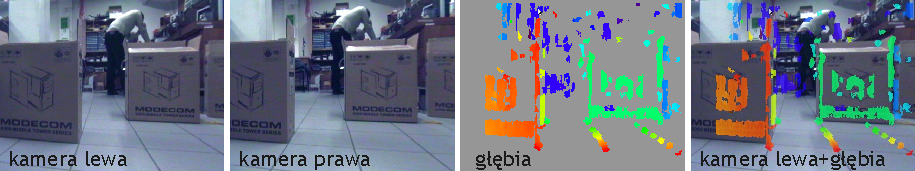
\includegraphics{../../Common/img/stereo_1}
\caption[Pierwsza scena testowa stereowizji]{Pierwsza scena testowa stereowizji.}
\label{fig:stereo_1}
\end{figure}

Scena na rysunku~\ref{fig:stereo_2} zawiera przeszkody pokryte bardziej zróżnicowaną
teksturą, dzięki czemu są one znacznie lepiej wykrywane, a mapa głębi jest bardziej
wypełniona.

Ostatni eksperyment (rysunek~\ref{fig:stereo_3}) miał na celu pokazanie problemu
przy wykrywaniu dużych, jednolitych obiektów. Tablica zajmuje dużą część obrazu
i stanowi poważną przeszkodę dla robota. Na mapie głębi jednak oznaczone są jedynie
jej boczne krawędzie, co mogłoby doprowadzić do próby przejazdu pomiędzy nimi.

\begin{figure}[h!]
\centering
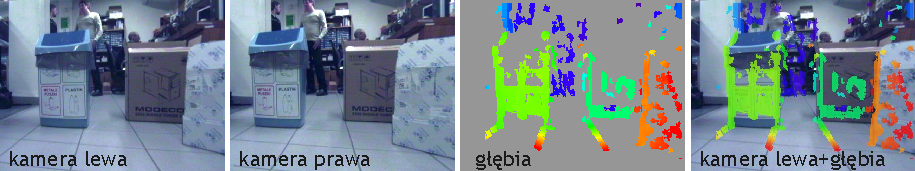
\includegraphics{../../Common/img/stereo_2}
\caption[Druga scena testowa stereowizji]{Druga scena testowa stereowizji zawierająca obiekty o zróżnicowanej teksturze.}
\label{fig:stereo_2}
\end{figure}

\begin{figure}[h!]
\centering
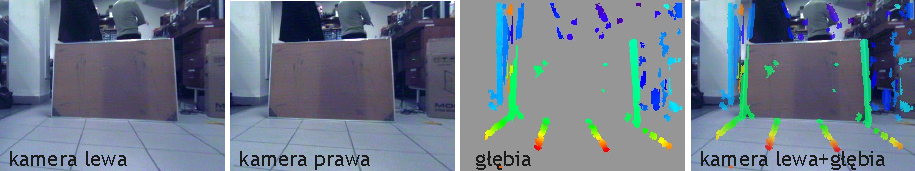
\includegraphics{../../Common/img/stereo_3}
\caption[Trzecia scena testowa stereowizji]{Trzecia scena testowa stereowizji pokazująca problemy z dużymi, jednolitymi przeszkodami.}
\label{fig:stereo_3}
\end{figure} 

%-------------------------------------------------------------------------------
\subsection{Światło strukturalne -- Microsoft Kinect}
%-------------------------------------------------------------------------------

Celem pomiarów było porównanie działania sensora Kinect i pary stereowizyjnej.
W tym celu przeanalizowano te same sceny, a obrazy wynikowe przedstawione są
poniżej. Największą różnicę widać w pokryciu obrazu na mapie głębi (w przypadku
Kinecta fragmenty nierozpoznane oznaczane są na czarno). Drugą różnicą, której
nie widać na obrazkach, jest prędkość działania. W przypadku sensora
firmy Microsoft algorytm jest zaimplementowany sprzętowo, co ma dwie zalety:
po pierwsze system komputera sterującego jest mniej obciążony, po drugie niezależnie
od jego obciążenia akwizycja danych działa z prędkością 30 klatek na sekundę.

\begin{figure}[h!]
\centering
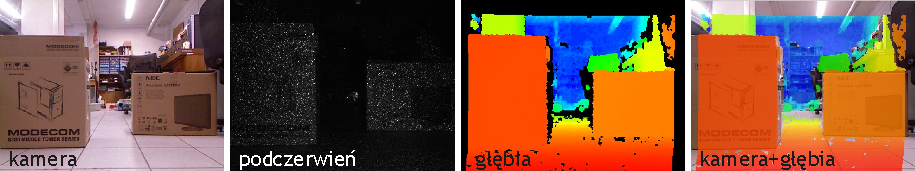
\includegraphics{../../Common/img/kinect_1}
\caption[Kinect -- pierwsza scena testowa]{Kinect -- pierwsza scena testowa}
\label{fig:kinect_1}
\end{figure}

Na rysunkach pokazany jest obraz z kamery RGB orazbraz widziany przez sensor
podczerwieni. Mapa głębi wyliczona na podstawie tego obrazu jest dodatkowo nakładana
na obraz RGB aby pokazać, w jaki sposób punkty z mapy głebi są skalibrowane z obrazem RGB.
Ogólnie dane dostarczane przez ten sensor są dużo lepszej jakości niż uzyskiwane
ze stereowizji, jednak istnieją przypadki trudne. Jednym z nich jest wykrywanie
wąskich, ciemnych przedmiotów (takich jak nogi od krzesła widoczne na
rysunku~\ref{fig:kinect_3}). Obiekty takie są zbyt małe, aby ich pokrycie przez
wzór referencyjny było odpowiednio duże, dodatkowo czarny kolor w dużym stopniu
pochłania światło podczerwone utrudniając ich lokalizację. W przypadku
korzystania ze stereowizji podobne przypadki nie stanowią problemu, ponieważ
wąskie, wyraźnie widoczne linie w obrazie są wykrywane jako punkty charakterystyczne
i są wykorzystywane w procesie tworzenia mapy dysparycji (można to zaobserwować
na rysunku~\ref{fig:stereo_3}, gdzie pomimo słabego wykrywania całej powierzchni
podłogi doskonale zaznaczane są czarne linie fug pomiędzy płytkami).

\begin{figure}[h!]
\centering
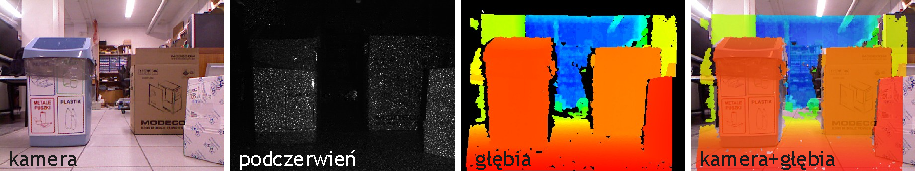
\includegraphics{../../Common/img/kinect_2}
\caption[Kinect -- druga scena testowa]{Kinect -- druga scena testowa}
\label{fig:kinect_2}
\end{figure}

\begin{figure}[h!]
\centering
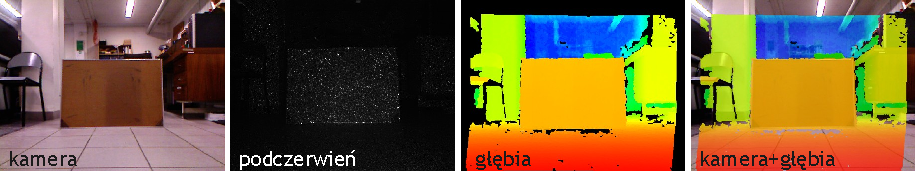
\includegraphics{../../Common/img/kinect_3}
\caption[Kinect -- trzecia scena testowa]{Kinect -- trzecia scena testowa}
\label{fig:kinect_3}
\end{figure}


% An example of a floating figure using the graphicx package.
% Note that \label must occur AFTER (or within) \caption.
% For figures, \caption should occur after the \includegraphics.
% Note that IEEEtran v1.7 and later has special internal code that
% is designed to preserve the operation of \label within \caption
% even when the captionsoff option is in effect. However, because
% of issues like this, it may be the safest practice to put all your
% \label just after \caption rather than within \caption{}.
%
% Reminder: the "draftcls" or "draftclsnofoot", not "draft", class
% option should be used if it is desired that the figures are to be
% displayed while in draft mode.
%
%\begin{figure}[!t]
%\centering
%\includegraphics[width=2.5in]{myfigure}
% where an .eps filename suffix will be assumed under latex,
% and a .pdf suffix will be assumed for pdflatex; or what has been declared
% via \DeclareGraphicsExtensions.
%\caption{Simulation Results}
%\label{fig_sim}
%\end{figure}

% Note that IEEE typically puts floats only at the top, even when this
% results in a large percentage of a column being occupied by floats.


% An example of a double column floating figure using two subfigures.
% (The subfig.sty package must be loaded for this to work.)
% The subfigure \label commands are set within each subfloat command, the
% \label for the overall figure must come after \caption.
% \hfil must be used as a separator to get equal spacing.
% The subfigure.sty package works much the same way, except \subfigure is
% used instead of \subfloat.
%
%\begin{figure*}[!t]
%\centerline{\subfloat[Case I]\includegraphics[width=2.5in]{subfigcase1}%
%\label{fig_first_case}}
%\hfil
%\subfloat[Case II]{\includegraphics[width=2.5in]{subfigcase2}%
%\label{fig_second_case}}}
%\caption{Simulation results}
%\label{fig_sim}
%\end{figure*}
%
% Note that often IEEE papers with subfigures do not employ subfigure
% captions (using the optional argument to \subfloat), but instead will
% reference/describe all of them (a), (b), etc., within the main caption.


% An example of a floating table. Note that, for IEEE style tables, the
% \caption command should come BEFORE the table. Table text will default to
% \footnotesize as IEEE normally uses this smaller font for tables.
% The \label must come after \caption as always.
%
%\begin{table}[!t]
%% increase table row spacing, adjust to taste
%\renewcommand{\arraystretch}{1.3}
% if using array.sty, it might be a good idea to tweak the value of
% \extrarowheight as needed to properly center the text within the cells
%\caption{An Example of a Table}
%\label{table_example}
%\centering
%% Some packages, such as MDW tools, offer better commands for making tables
%% than the plain LaTeX2e tabular which is used here.
%\begin{tabular}{|c||c|}
%\hline
%One & Two\\
%\hline
%Three & Four\\
%\hline
%\end{tabular}
%\end{table}


% Note that IEEE does not put floats in the very first column - or typically
% anywhere on the first page for that matter. Also, in-text middle ("here")
% positioning is not used. Most IEEE journals/conferences use top floats
% exclusively. Note that, LaTeX2e, unlike IEEE journals/conferences, places
% footnotes above bottom floats. This can be corrected via the \fnbelowfloat
% command of the stfloats package.


% trigger a \newpage just before the given reference
% number - used to balance the columns on the last page
% adjust value as needed - may need to be readjusted if
% the document is modified later
%\IEEEtriggeratref{8}
% The "triggered" command can be changed if desired:
%\IEEEtriggercmd{\enlargethispage{-5in}}

% references section

% can use a bibliography generated by BibTeX as a .bbl file
% BibTeX documentation can be easily obtained at:
% http://www.ctan.org/tex-archive/biblio/bibtex/contrib/doc/
% The IEEEtran BibTeX style support page is at:
% http://www.michaelshell.org/tex/ieeetran/bibtex/
\bibliographystyle{IEEEtran}
% argument is your BibTeX string definitions and bibliography database(s)
\bibliography{IEEEabrv,mybib}
%
% <OR> manually copy in the resultant .bbl file
% set second argument of \begin to the number of references
% (used to reserve space for the reference number labels box)

%\begin{thebibliography}{1}
%
%\bibitem{IEEEhowto:kopka}
%H.~Kopka and P.~W. Daly, \emph{A Guide to \LaTeX}, 3rd~ed.\hskip 1em plus
%  0.5em minus 0.4em\relax Harlow, England: Addison-Wesley, 1999.
%
%\end{thebibliography}




% that's all folks
\end{document}


